\documentclass[tikz,14pt,fleqn]{article}

% Math
\usepackage[fleqn]{amsmath}
\usepackage{amssymb}
\usepackage{dsfont}
\usepackage{float}

% Insert dummy text
\usepackage{lipsum}  
% Allows to use caption*
\usepackage{caption}
% Scalabale subfigures
\usepackage{subcaption} 
% Code syntax highlighting
\usepackage{minted}
% Hyperlinks
\usepackage{hyperref}
% Customize page layout
\usepackage{geometry}
\geometry{a4paper, margin=1in}
% Page headers and footers
\usepackage{fancyhdr}
\pagestyle{fancy}
\fancyhf{}
\setlength{\parindent}{0pt}
\setlength{\parskip}{0.5\baselineskip}%

% includegraphics
\usepackage{graphicx}




\newcommand{\bmat}[1]{
   \ensuremath{
   \begin{bmatrix}
       #1
   \end{bmatrix}
}}




\usepackage[utf8]{inputenc}


%%%%%%%%%%%%%%%%%%%%%%%%%%%%
%% VARIABLES
\newcommand\namesurname{Albert Cerfeda}
\newcommand\assignment{Assignment 1}

\newcommand\subject{Image \& Video Processing}
\newcommand\documentdate{19 March 2023}

% Title content
%%%%%%%%%%%%%%%%%%%%%%%%%%%%
\rhead{\assignment}
\lhead{\namesurname}
%%%%%%%%%%%%%%%%%%%%%%%%%%%%

\rfoot{Page \thepage}


\begin{document}

\begin{titlepage}
   \begin{center}
       \vspace*{0.2cm}

       \textbf{\Large{\subject}}

       \vspace{0.5cm}
        \textbf{\assignment}\\[5mm]
        
            
       \vspace{0.4cm}

        \namesurname
        \begin{figure}[H]
            \centering
        \end{figure}
       \tableofcontents

       \vspace*{\fill}
     
        
\includegraphics[width=0.4\textwidth]{fig/logo.png}
       
        \documentdate \\
        Università della Svizzera italiana\\
        Faculty of Informatics\\
        Switzerland\\

   \end{center}
\end{titlepage}

\section{Point Operations [20 points]}


\subsection{Tone mapping \& Linearization [2 points]}
 The provided image $\texttt{ferrari.jpg}$ has been gamma corrected in order to take into account the non-linear conversion from intensity value to the actual emitted light on the screen.
In this exercise we perform various transformations on the provided image:
 \begin{itemize}
    \item Linearize the image back by inverting the gamma correction.\\
    We know that the image has been encoded with gamma $\gamma = \frac{1}{2.2}$, so the inverse operation is to raise the intensity values to the power of $\gamma = 2.2$. Results are shown in Figure \ref{fig:1.ferrari_lin}.
    \item Increase the brightness of the image by multiplying the intensity values by a constant factor.\\
    Let us increase the brightness by a factor of 2. Results are shown in Figure \ref{fig:1.ferrari_bri}.
    \item Enhance the contrast of the image by applying an exponential function to the intensity values. Results are shown in Figure \ref{fig:1.ferrari_con}.
 \end{itemize}
 \begin{minted}[frame=lines, framesep=1.5mm, fontsize=\small]{matlab} 
im_lin = im.^2.2; % 1.1 Linearize the image
im_lin = im.*2;   % 1.2 Increase the brightness
im_con = im.^0.7; % 1.3 Enhance the contrast
\end{minted}

\begin{figure}[h!]
\begin{center}
    \begin{subfigure}{0.38\textwidth}
        \centering
        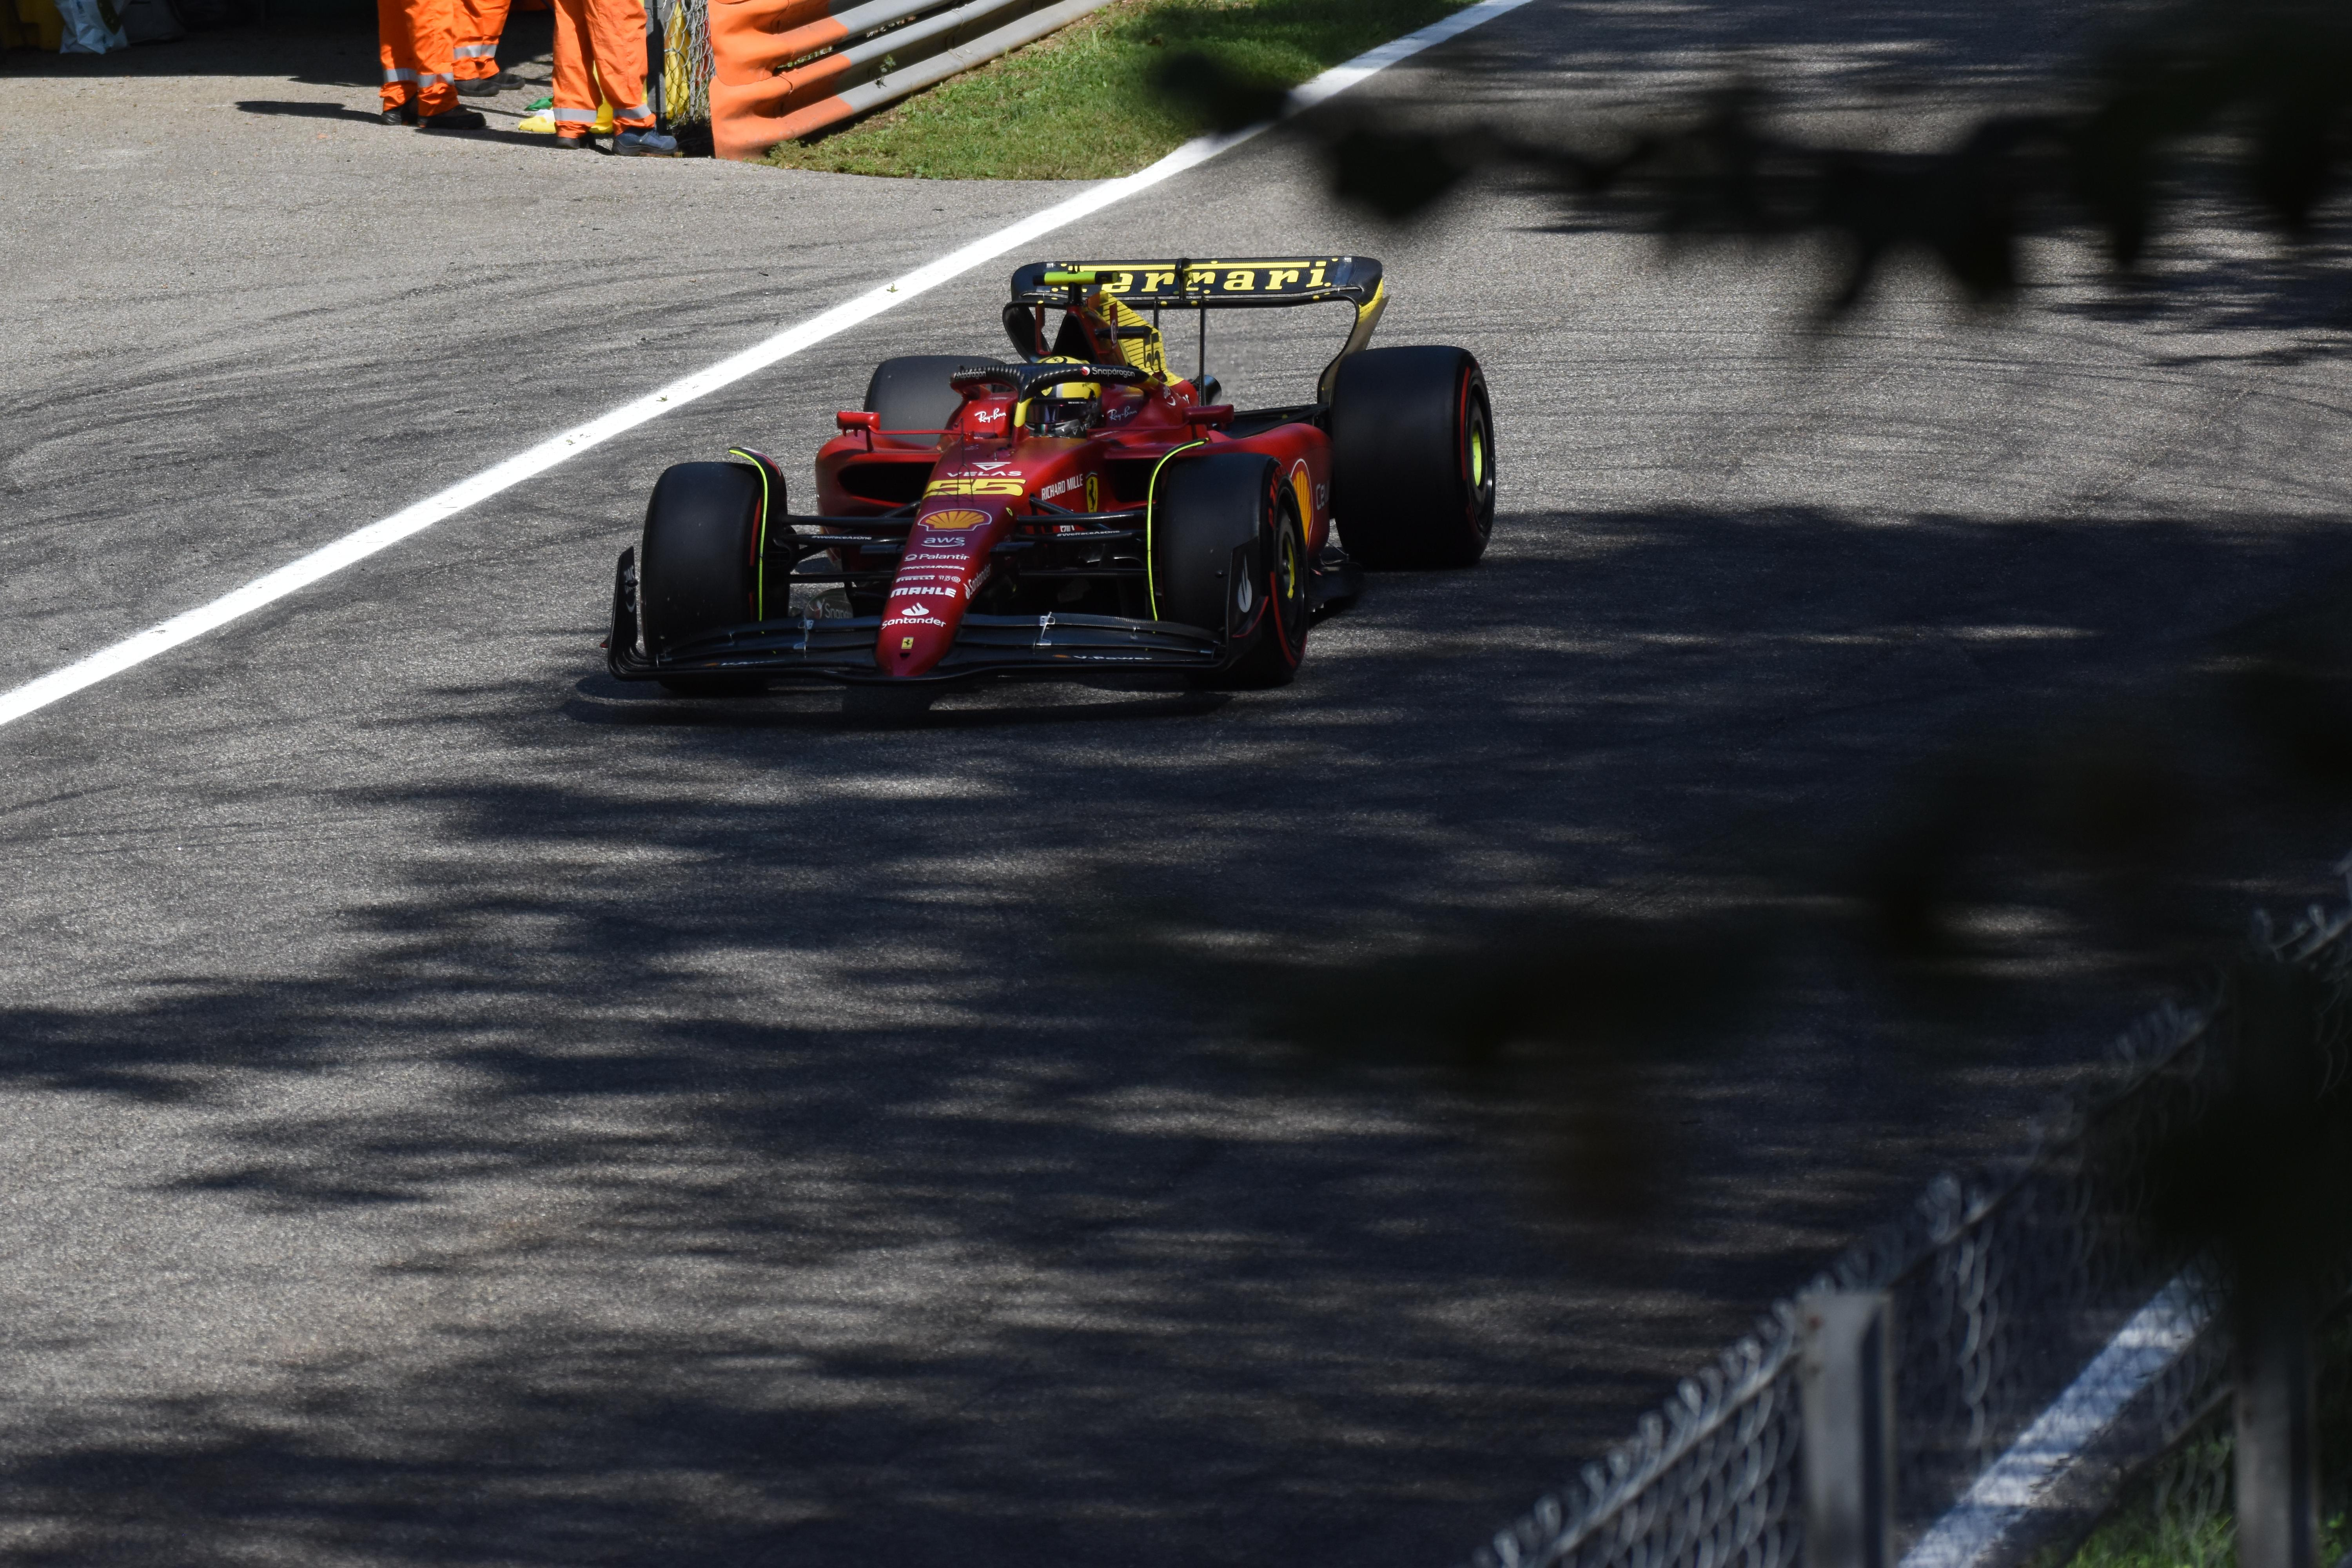
\includegraphics[width=\textwidth]{fig/out/1.ferrari.jpg}
        \caption{Original $\texttt{ferrari.jpg}$.}
    \end{subfigure}
    \begin{subfigure}{0.38\textwidth}
        \centering
        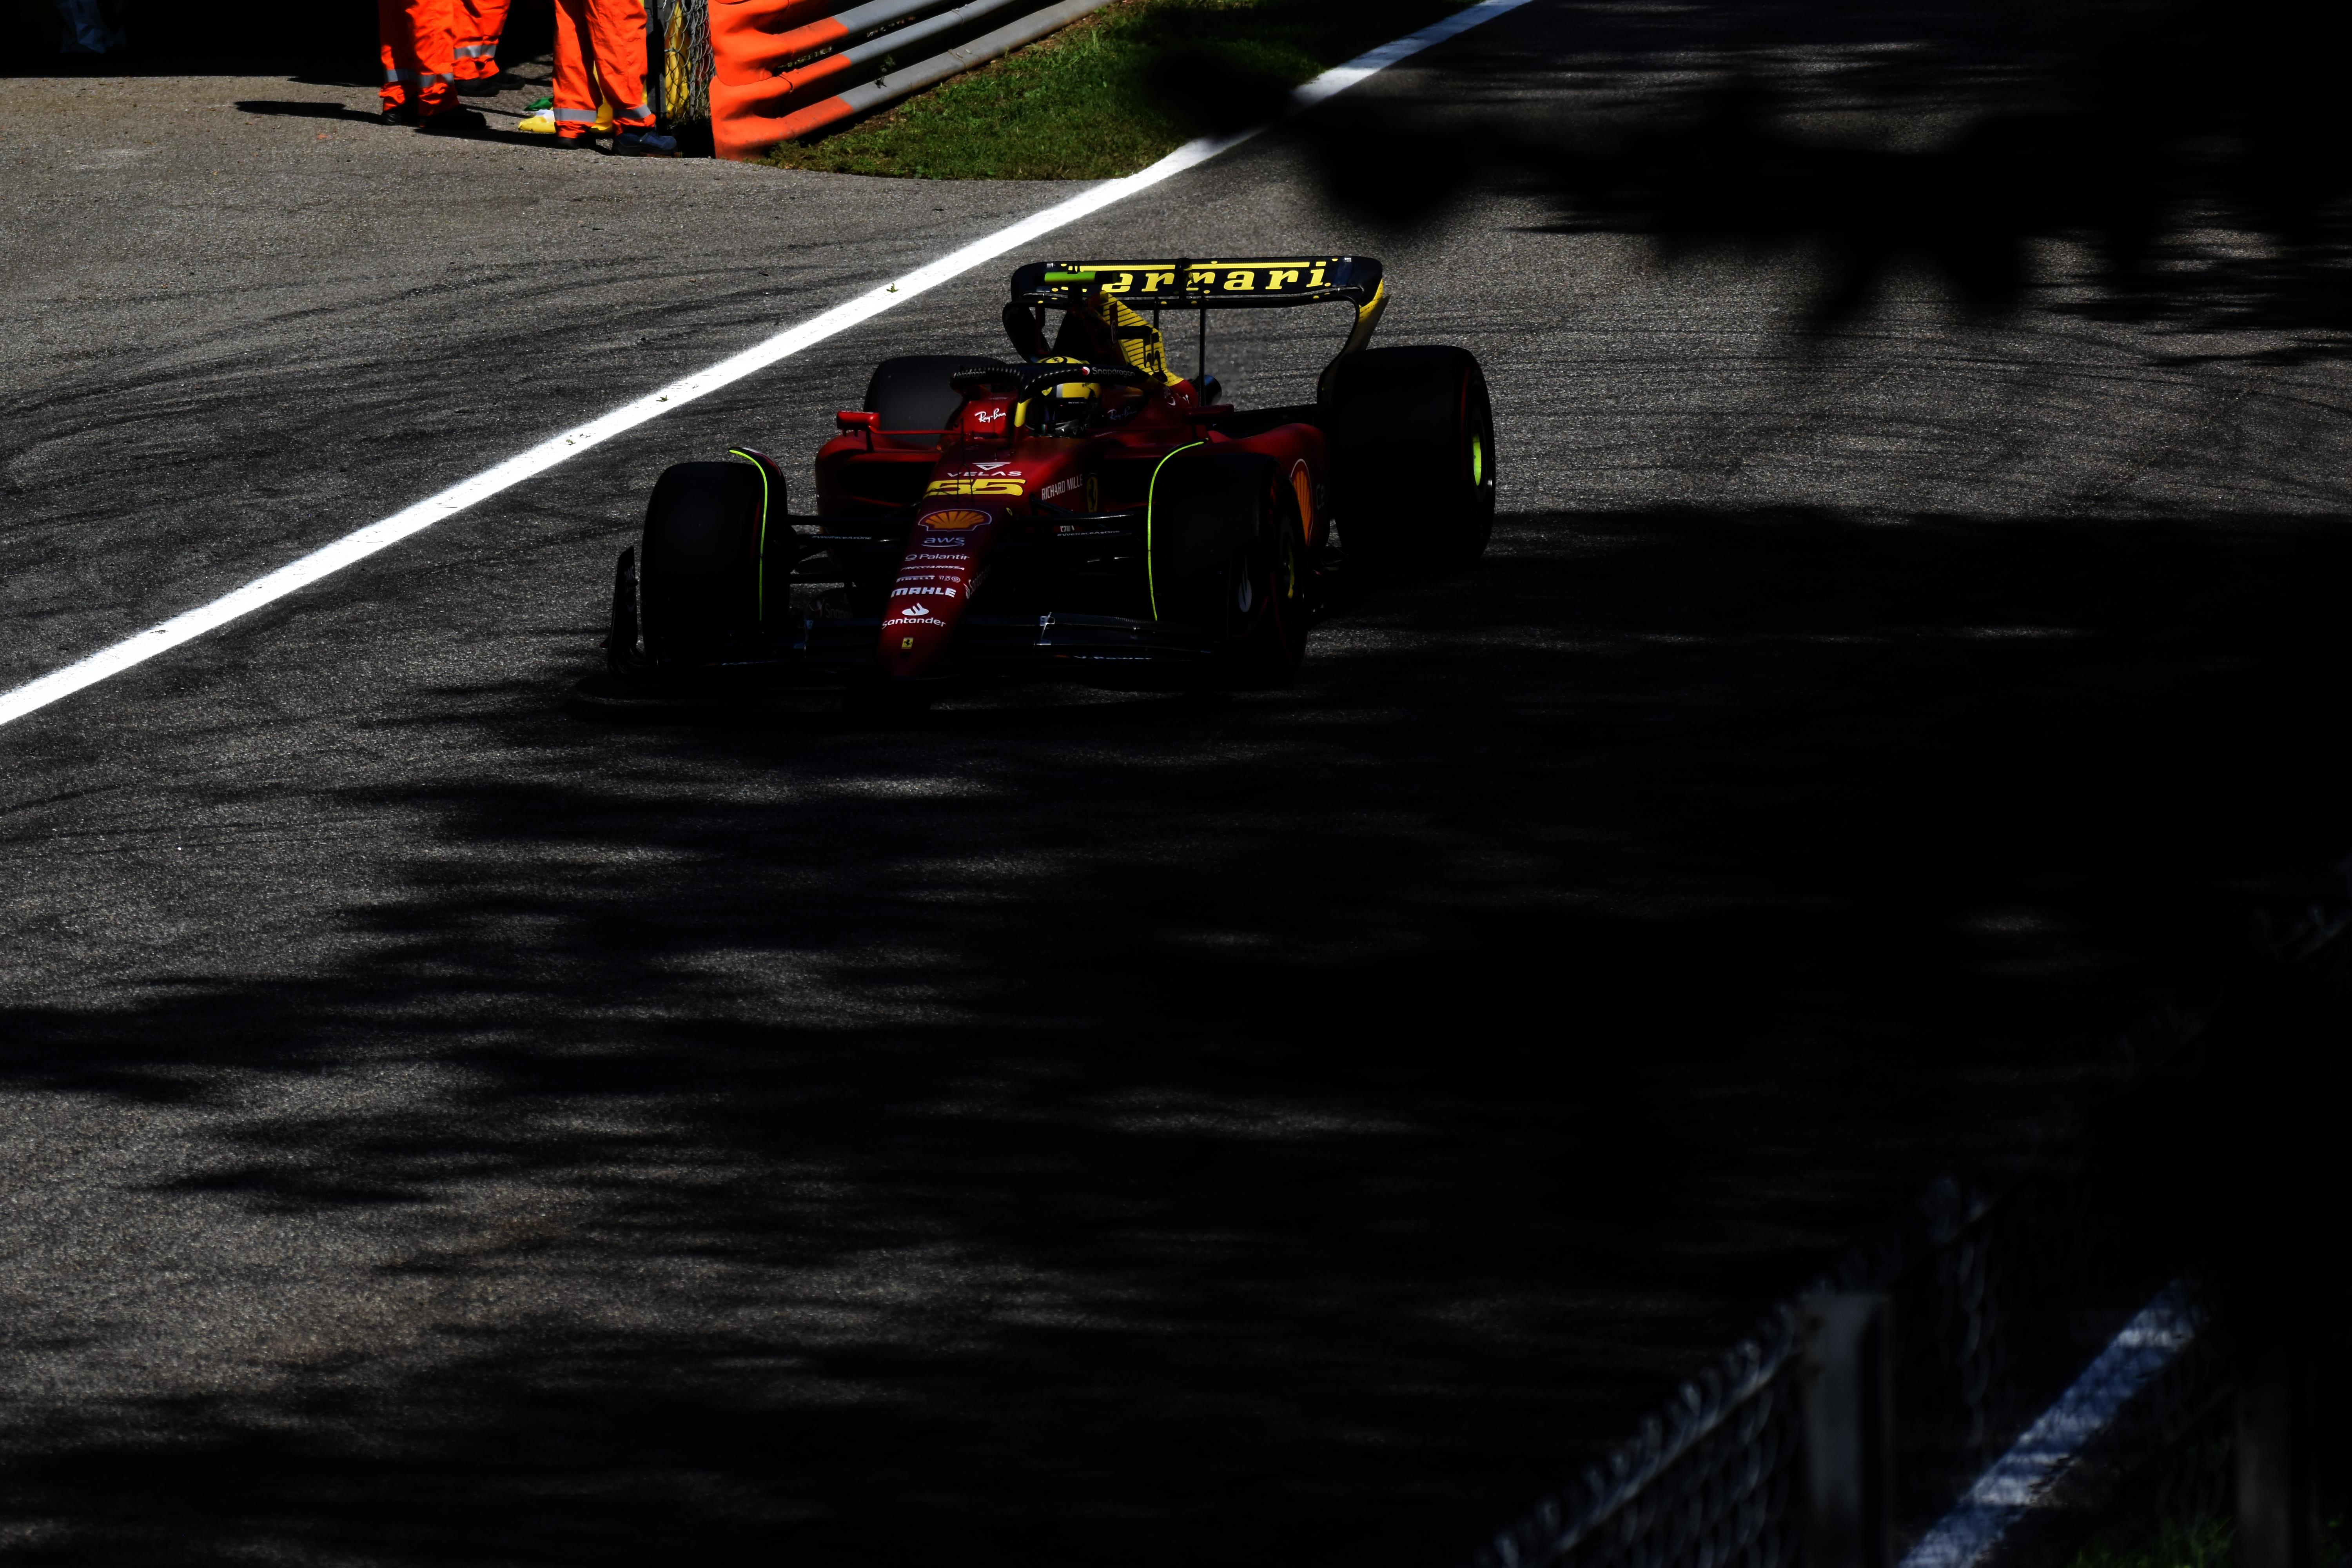
\includegraphics[width=\textwidth]{fig/out/1.ferrari_lin.jpg}
        \caption{$\texttt{ferrari\_lin.jpg}$. Linearized contrast}
        \label{fig:1.ferrari_lin}
    \end{subfigure}
% \end{center}
% \begin{center}
    \begin{subfigure}{0.38\textwidth}
        \centering
        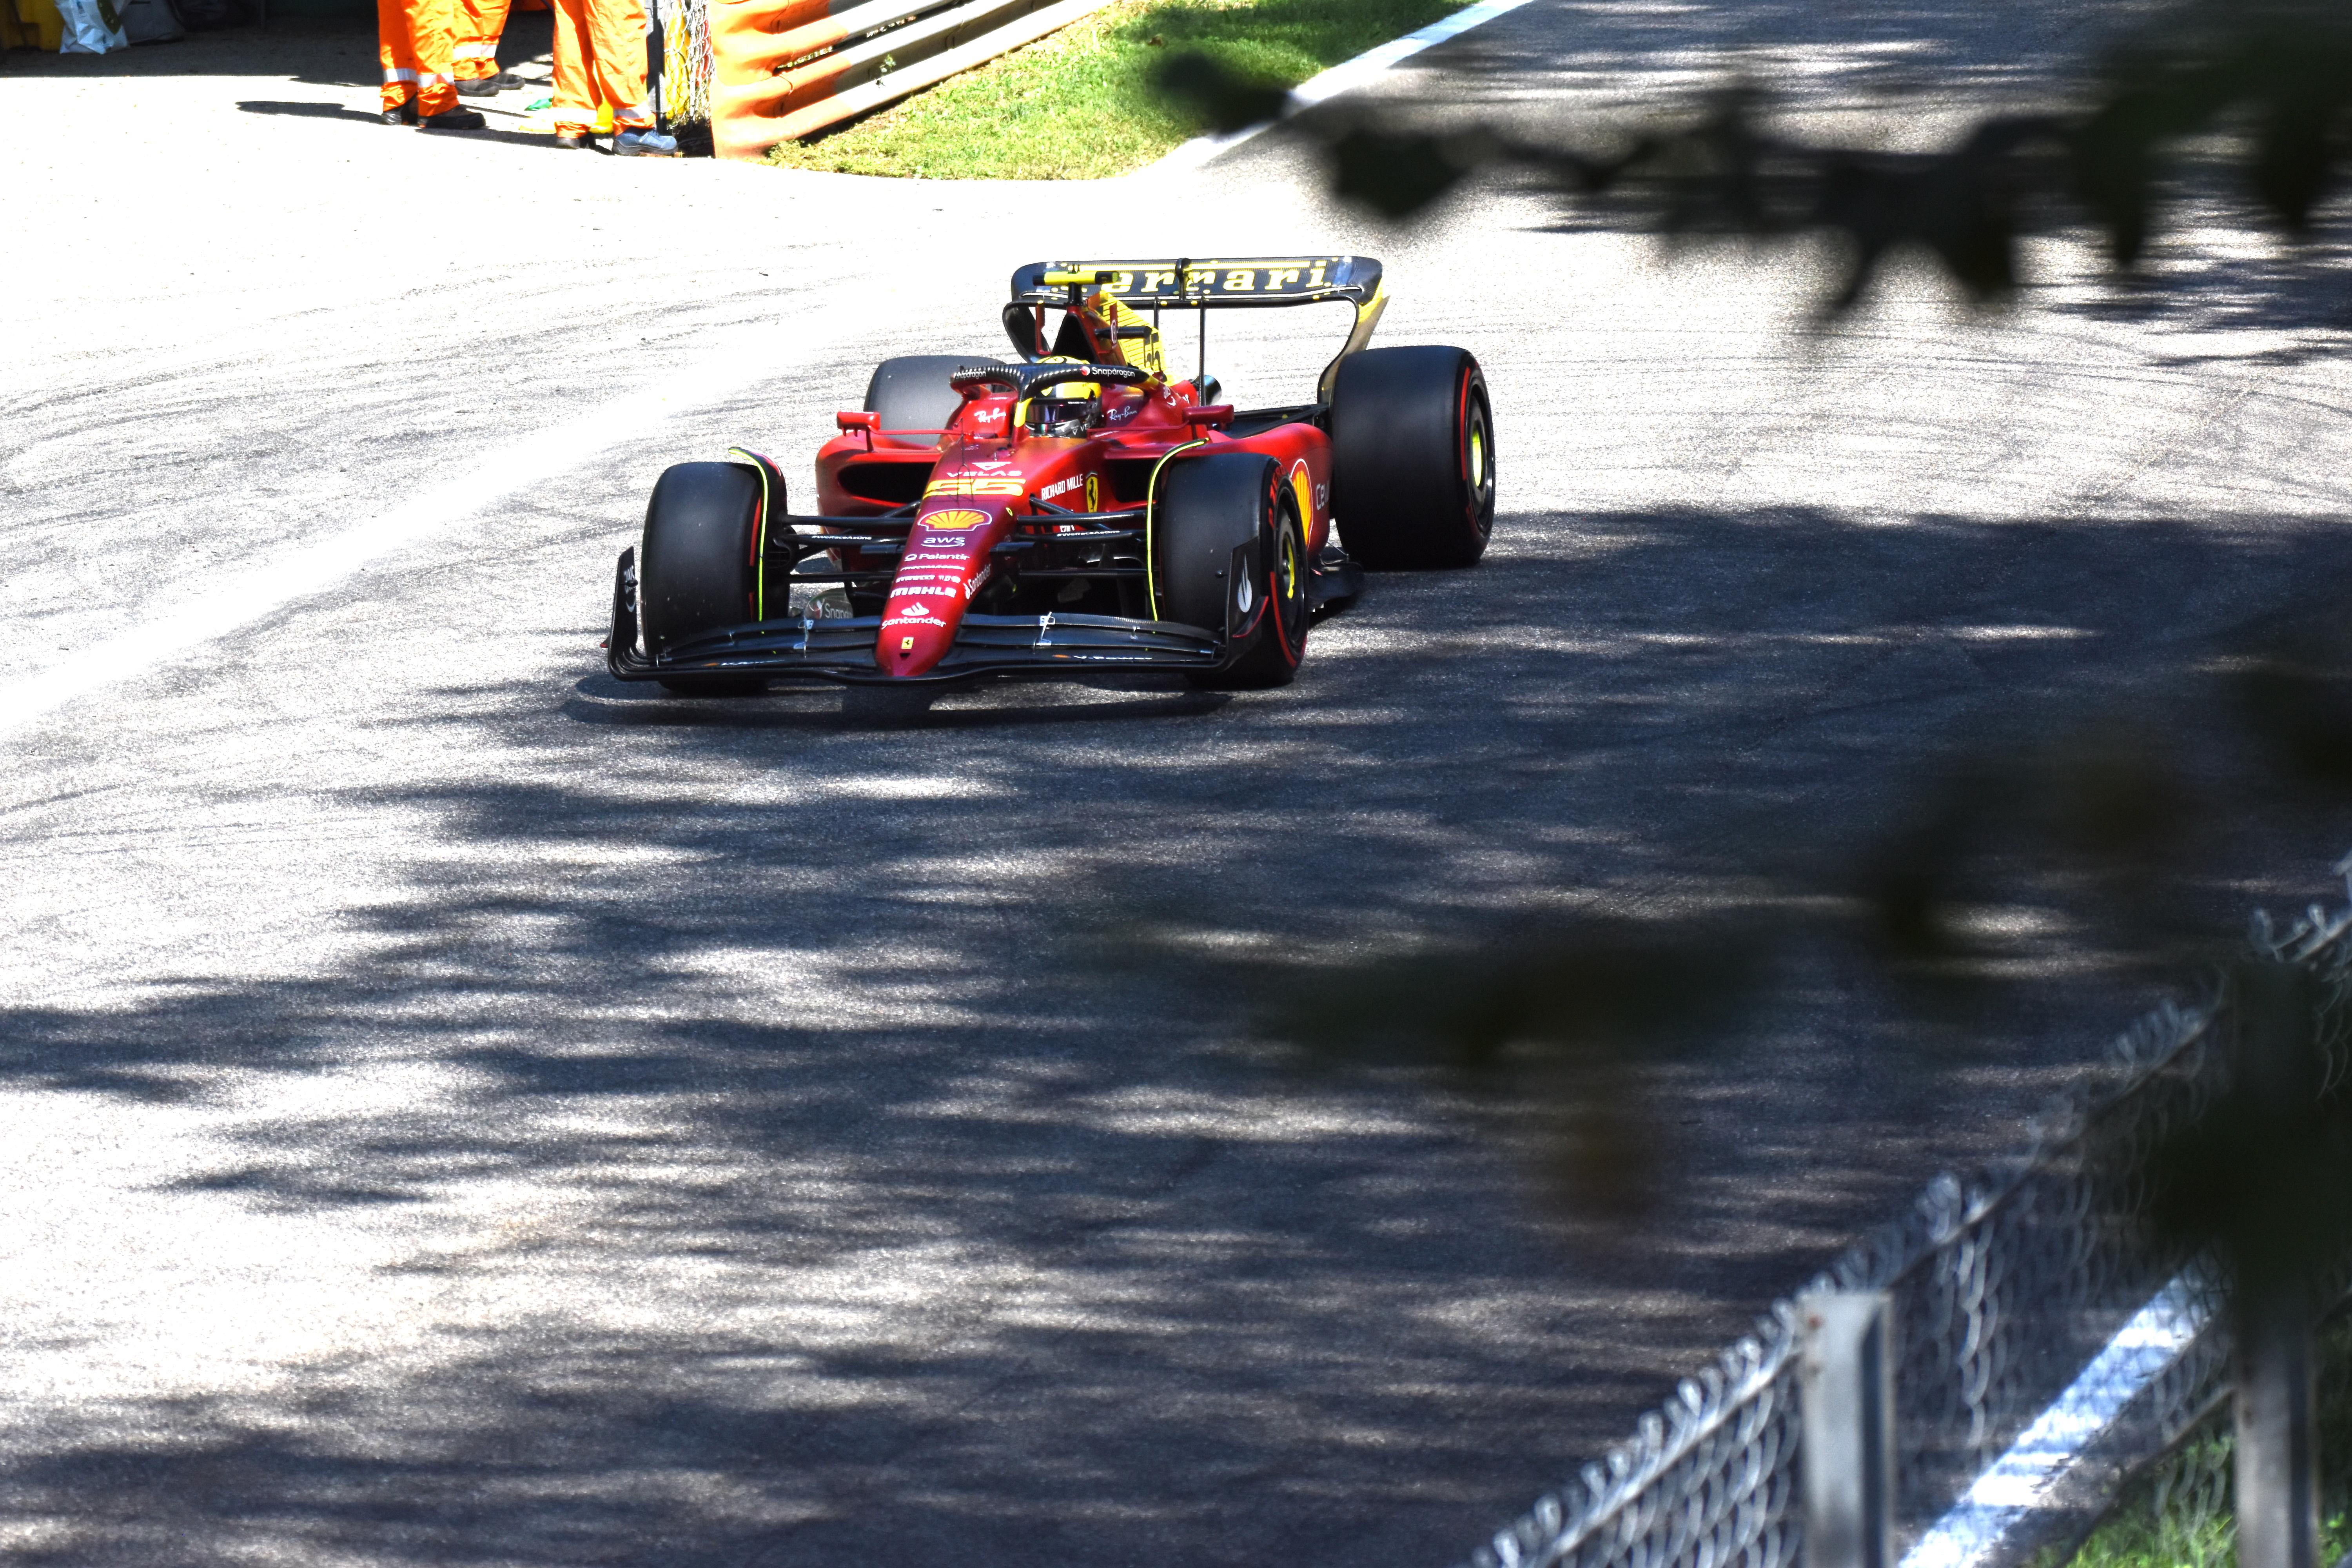
\includegraphics[width=\textwidth]{fig/out/1.ferrari_bri.jpg}
        \caption{$\texttt{ferrari\_bri.jpg}$. Scaled brightness}
        \label{fig:1.ferrari_bri}
    \end{subfigure}
    \begin{subfigure}{0.38\textwidth}
        \centering
        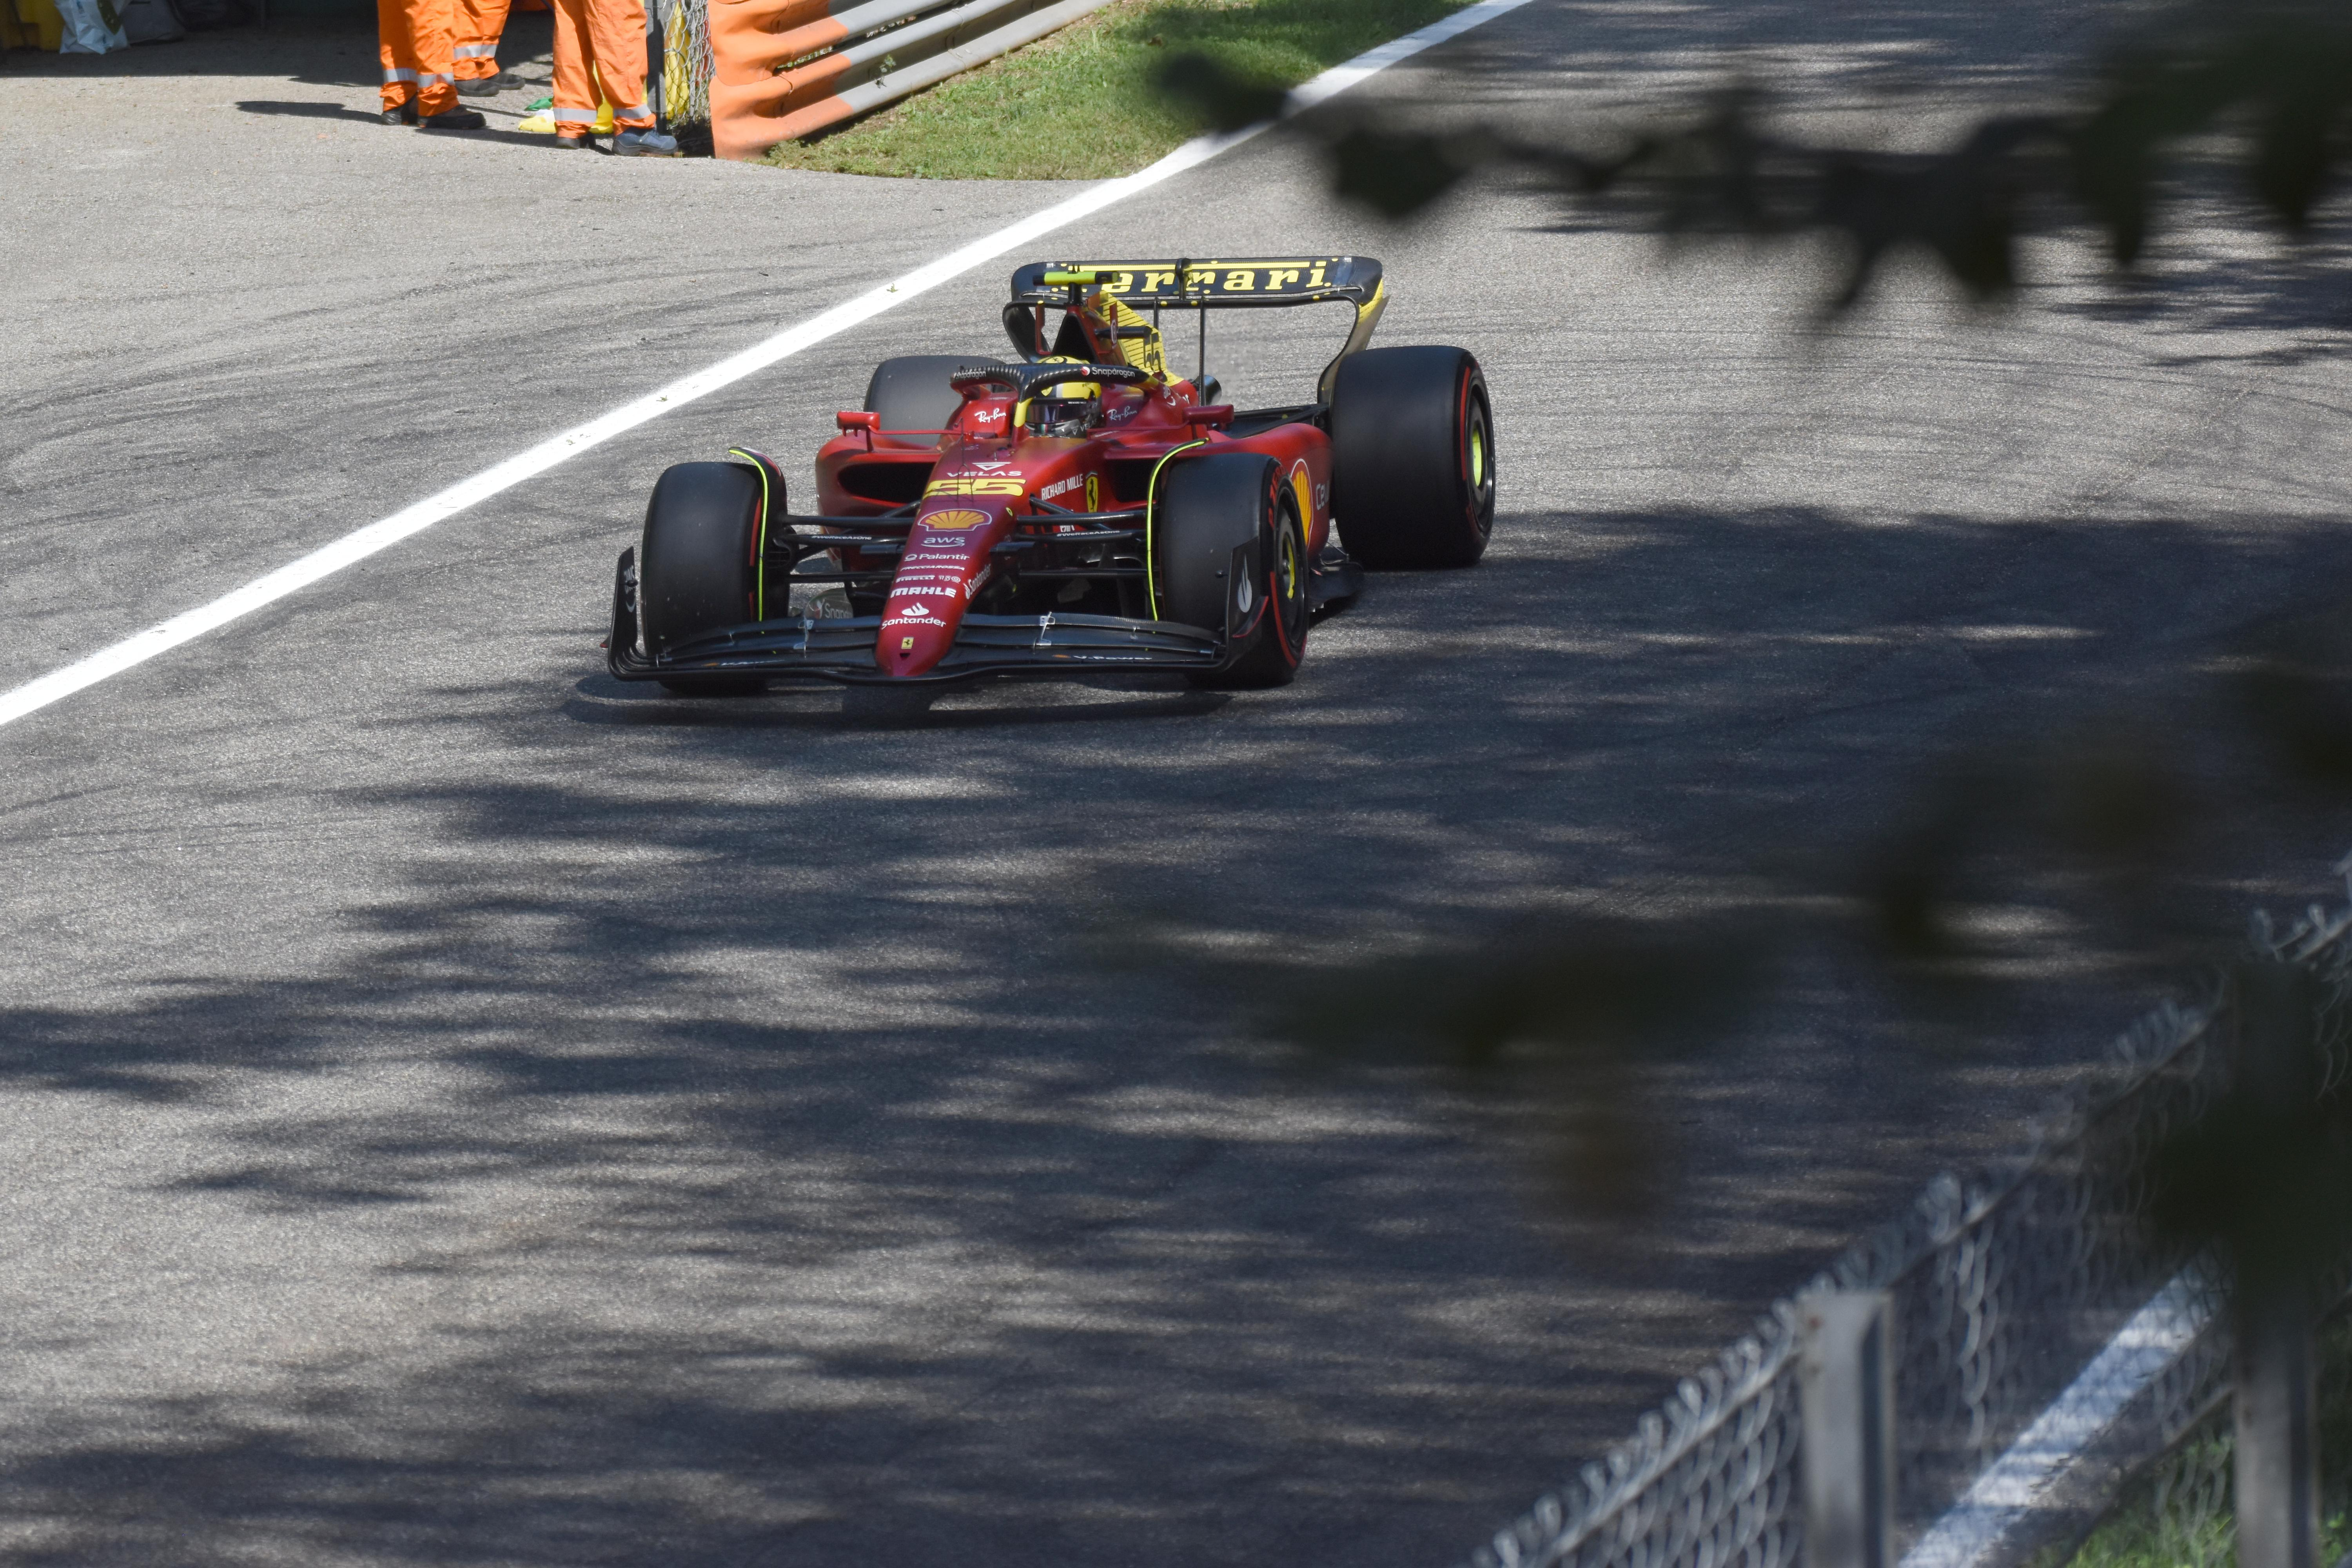
\includegraphics[width=\textwidth]{fig/out/1.ferrari_con.jpg}
        \caption{$\texttt {ferrari\_con.jpg}$. Exponential contrast.}
        \label{fig:1.ferrari_con}
    \end{subfigure}

    \caption{Tonemapping procedure comparison.}
    \label{fig:1.results}
\end{center}

\end{figure}
\subsection{Color correction [4 points]}
During image acquisition, the color of the light sources affect the color of the captured image. Our eyes, unlike cameras, are able to adapt to the color of the light source and thus we are able to see the correct colors. In order to represent the colors as they are seen by our eyes, we need to perform white balancing. We implement different white-balancing transformations:
\begin{itemize}
    \item Pixel-based correction\\
    We choose a pixel in the image that appears gray, and we balance the color channels around the chosen pixel's color. Results are shown in Figure \ref{fig:2.wb_pxcorr}.
    \item Gray-world assumption\\
    We assume that the average color of the image is gray so, instead of balancing the image colors around some pixel, we balance the channel mean itself. Results are shown in Figure \ref{fig:2.wb_gwa}. We can notice how this method is the most effective when it comes to neutralize the blue tint given by the light source.
\end{itemize}
\begin{figure}[h!]
    \begin{minted}[frame=lines, framesep=2mm, linenos, fontsize=\small ]{matlab} 
% ...
channelmean = mean(mean(im))

% 2.1 Pixel-based correction
figure(); imshow(im);
coords = int32(ginput(1));
px_color = im(coords(2), coords(1), 1:3);
gain = px_color./channelmean;
im_pxcorr = im.*gain;

% 2.2 Gray-world assumption
gain = channelmean/mean(channelmean);
im_gwa = im./gain;
        \end{minted}
\caption{Matlab code performing various intensity transformations on the image $\texttt{ferrari.jpg}$.}
\end{figure}
\begin{figure}[h!]
    \begin{center}
    \begin{subfigure}{0.31\linewidth}
        \centering
        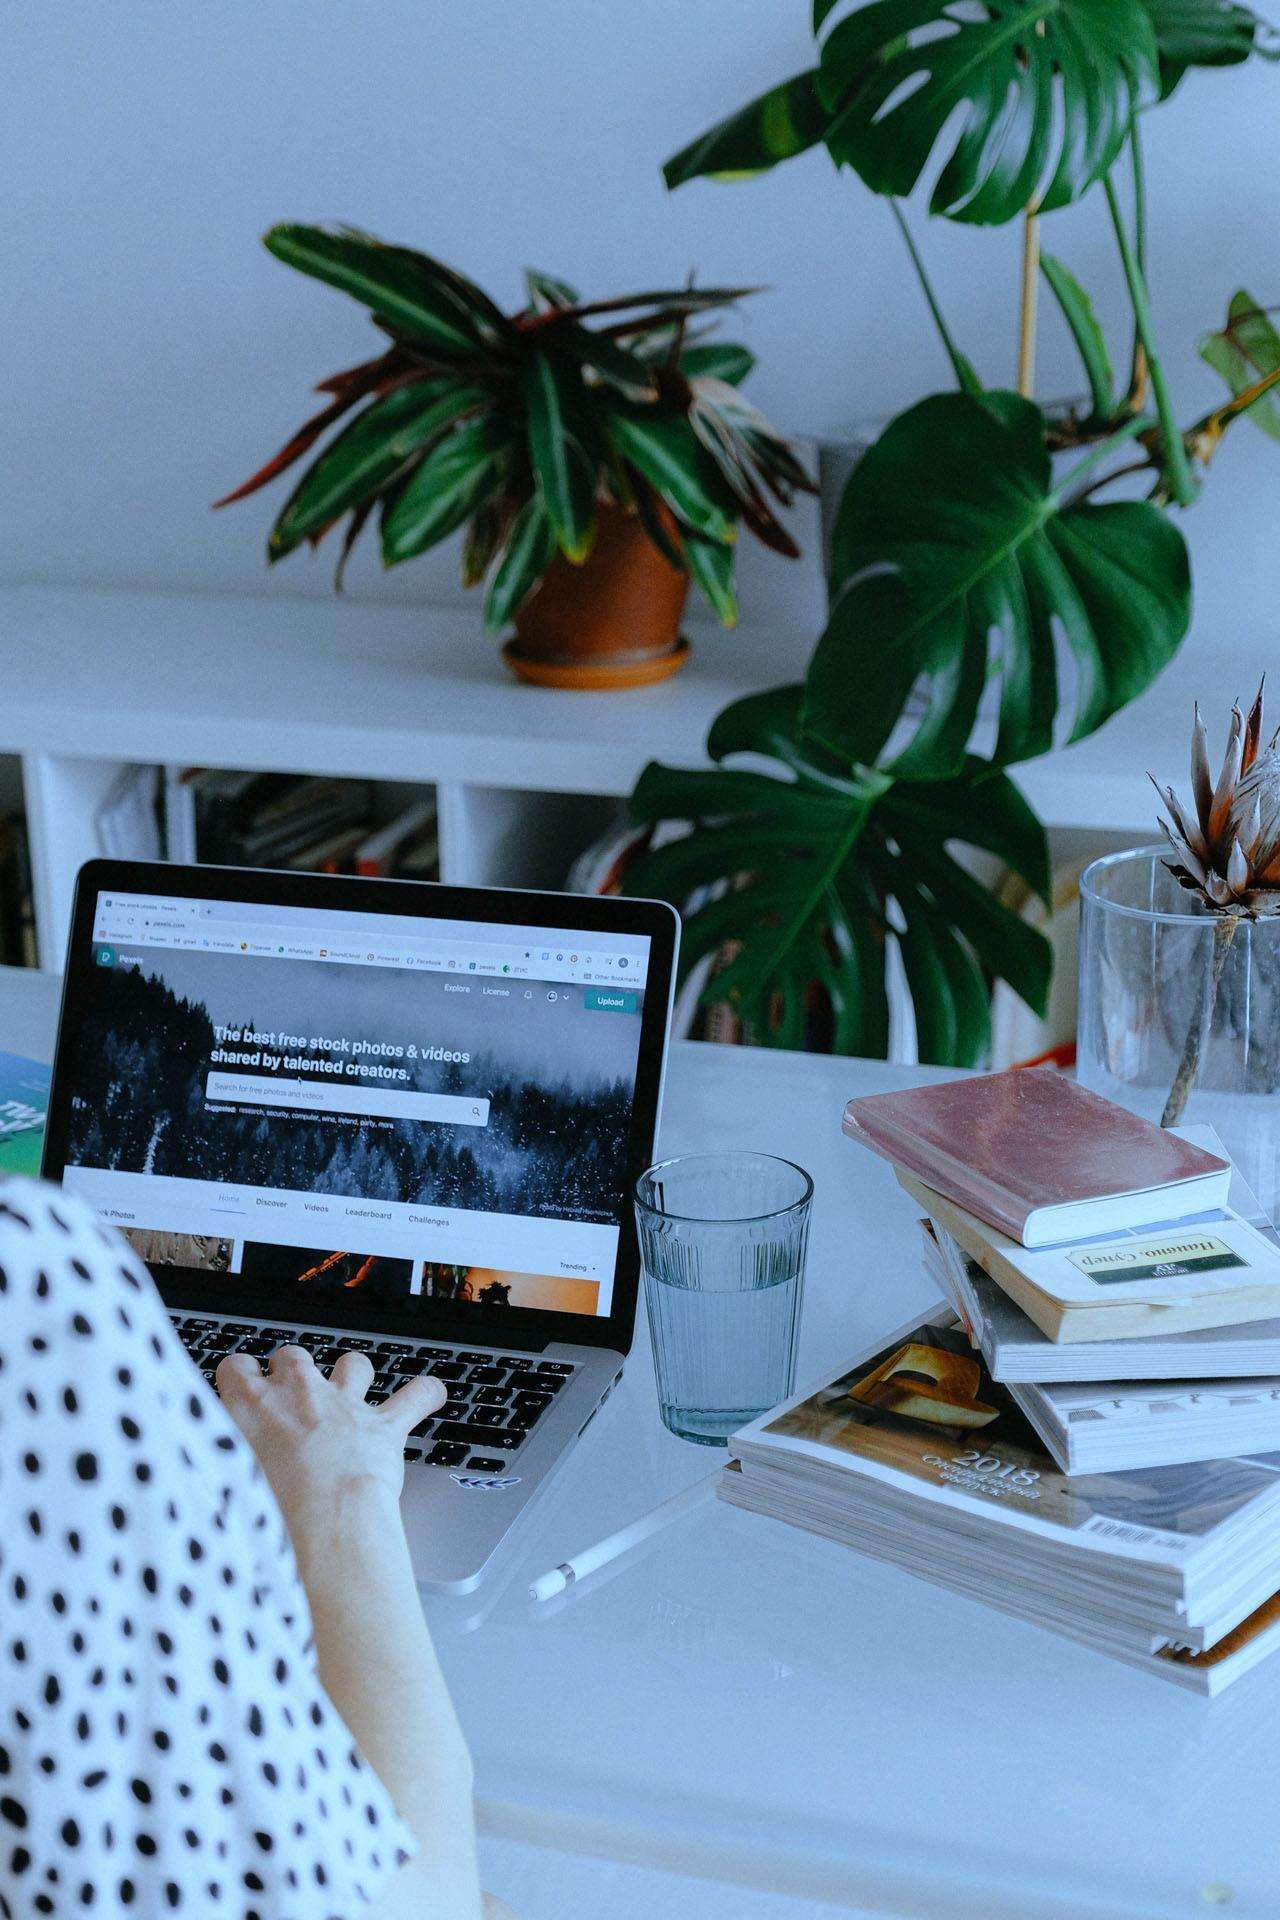
\includegraphics[width=\linewidth]{fig/out/2.wb.jpg}
        \caption{Original image}
        \label{fig:2.wb}
    \end{subfigure}
    \begin{subfigure}{0.31\linewidth}
        \centering
        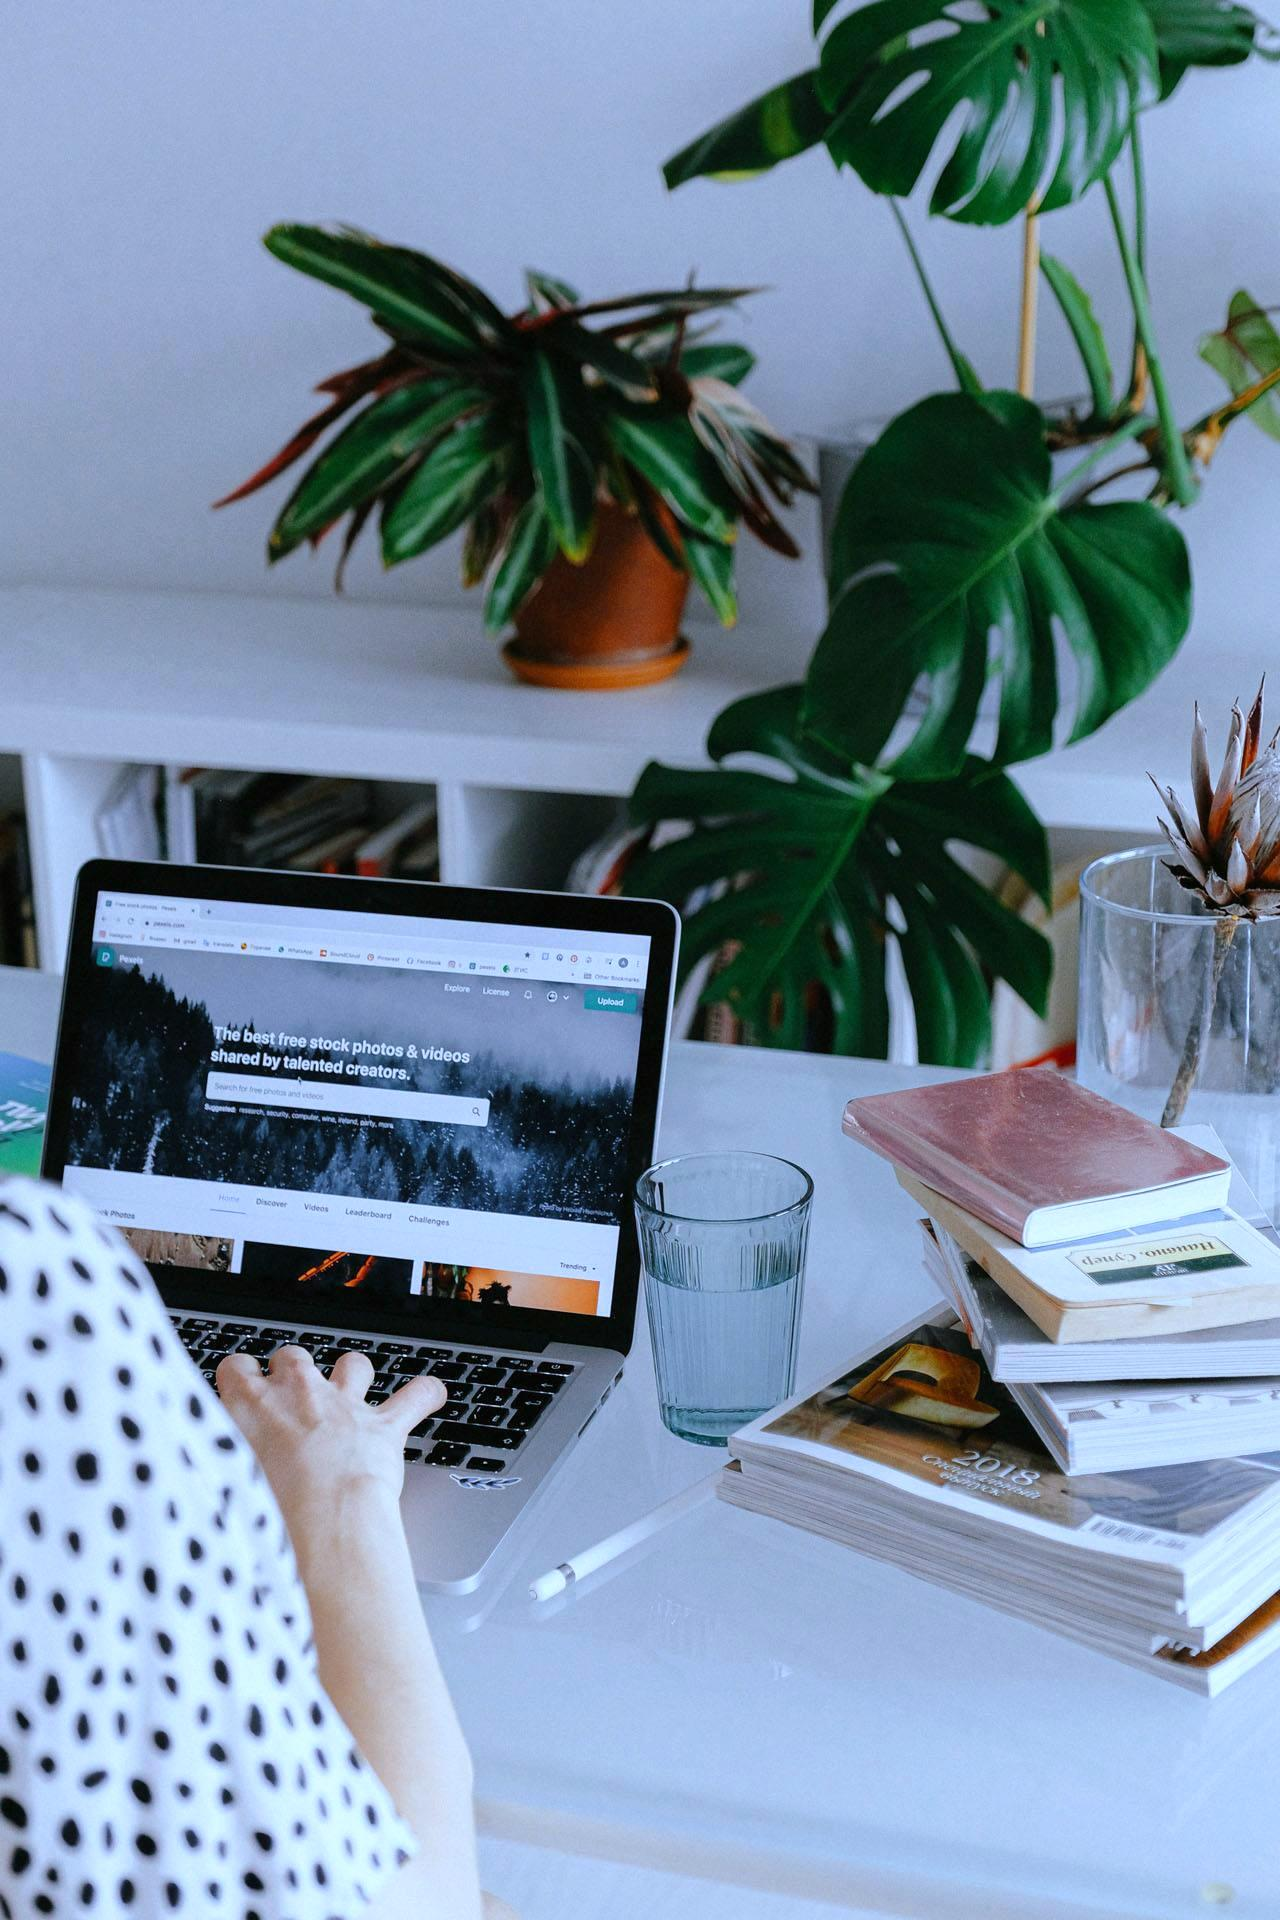
\includegraphics[width=\linewidth]{fig/out/2.wb_pxcorr.jpg}
        \caption{Pixel-based correction}
        \label{fig:2.wb_pxcorr}
    \end{subfigure}
    \begin{subfigure}{0.31\linewidth}
        \centering
        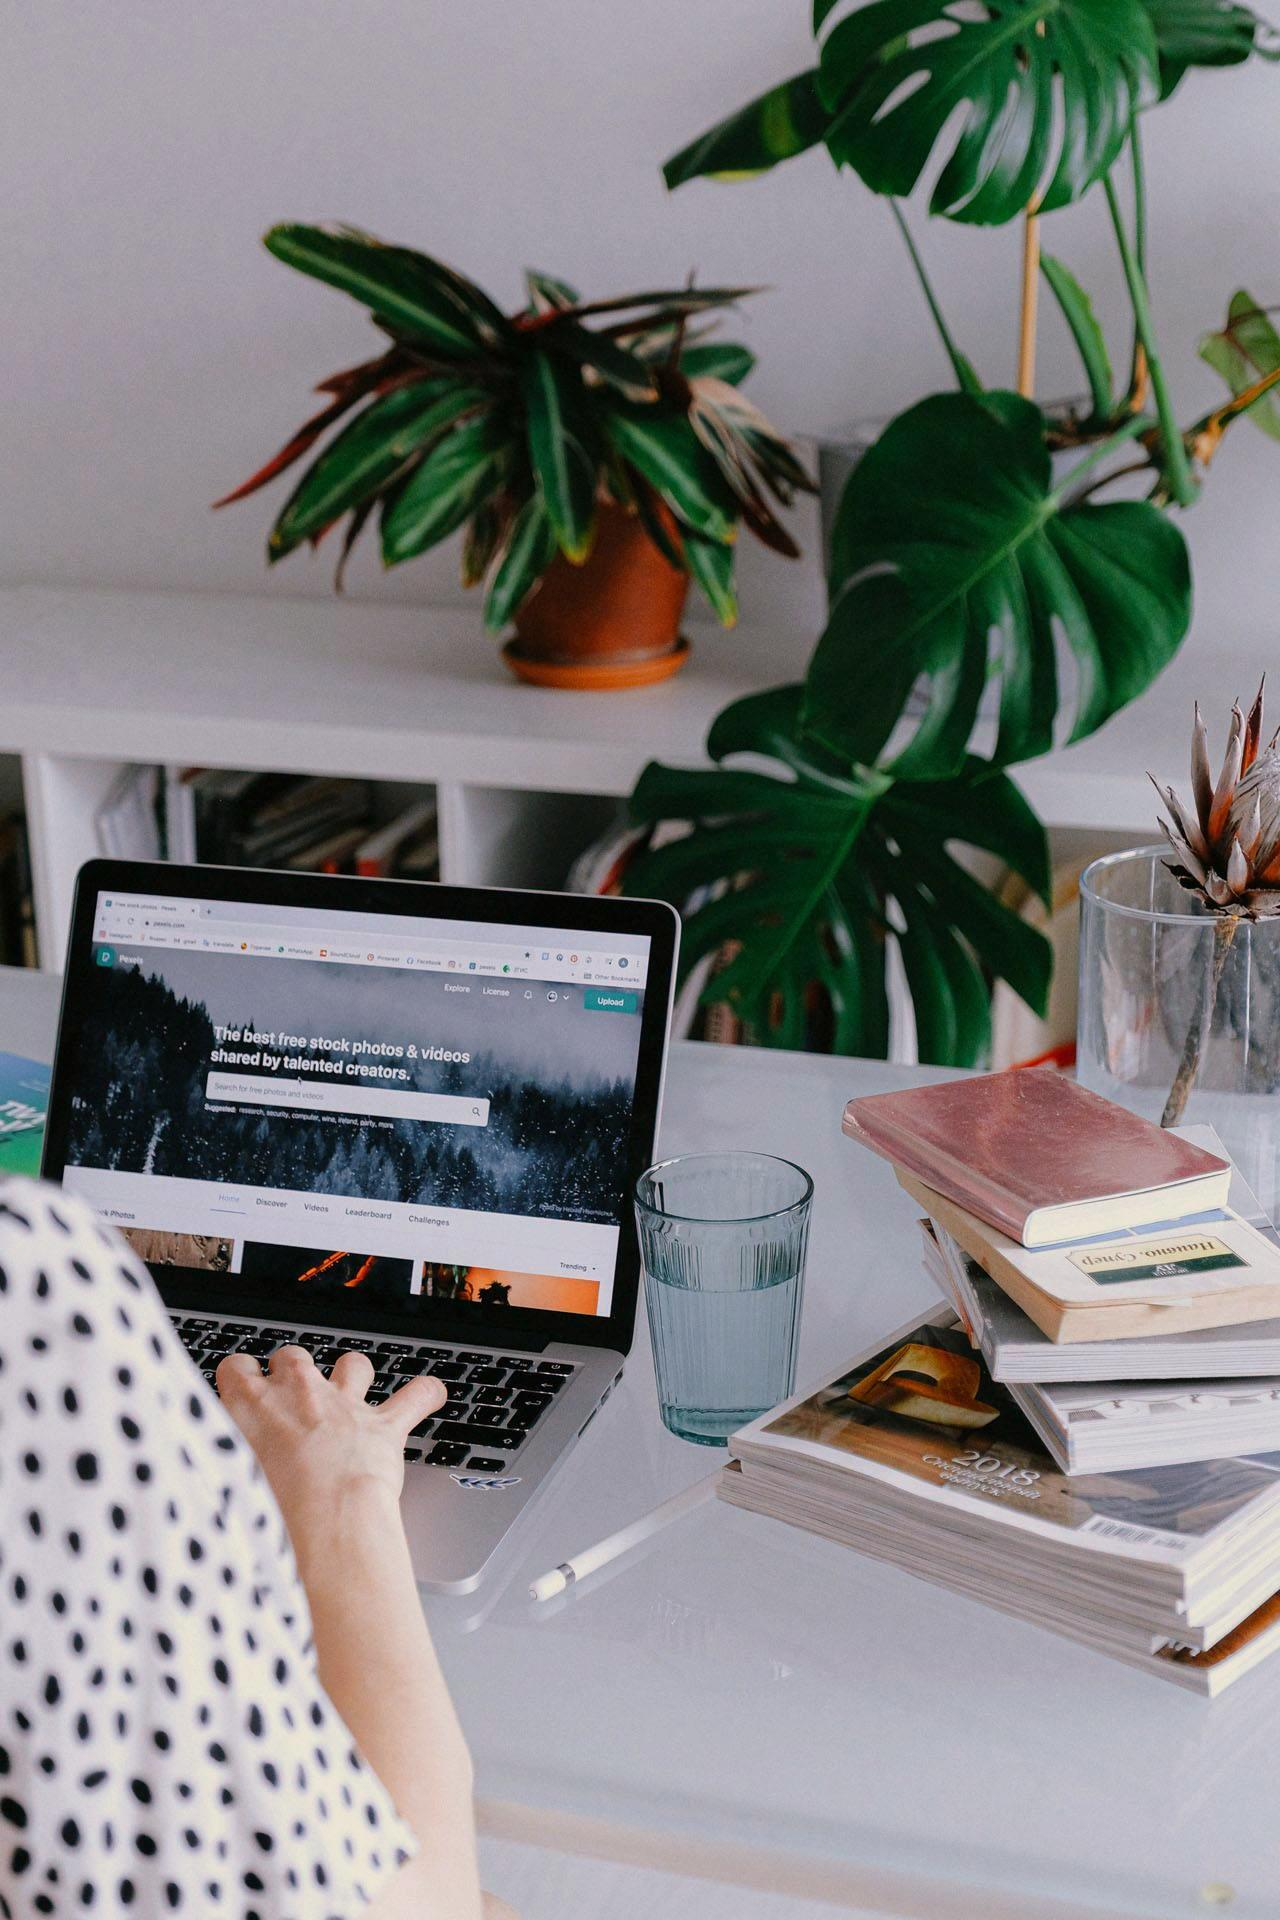
\includegraphics[width=\linewidth]{fig/out/2.wb_gwa.jpg}
        \caption{Gray-world assumption correction}
        \label{fig:2.wb_gwa}
    \end{subfigure}
    \caption{Color correction procedures comparison.}
\end{center}
\end{figure}
\subsection{Histograms [1 point]}
Image histograms show us the distribution of the different pixel values for each color channel. Let us implement a function to compute RGB image histograms.
\begin{minted}[frame=lines, fontsize=\small]{matlab}
function [distribution] = compute_distribution(channel)
    distribution = cell2mat(arrayfun(@(x) sum(sum(channel==x)), 0:255,'UniformOutput',false));
end
\end{minted}
In the implementation, every intensity value in the \verb|0:255| range gets mapped to the number of occurrences of the value in the channel.
\begin{figure}[h!]
    \centering
    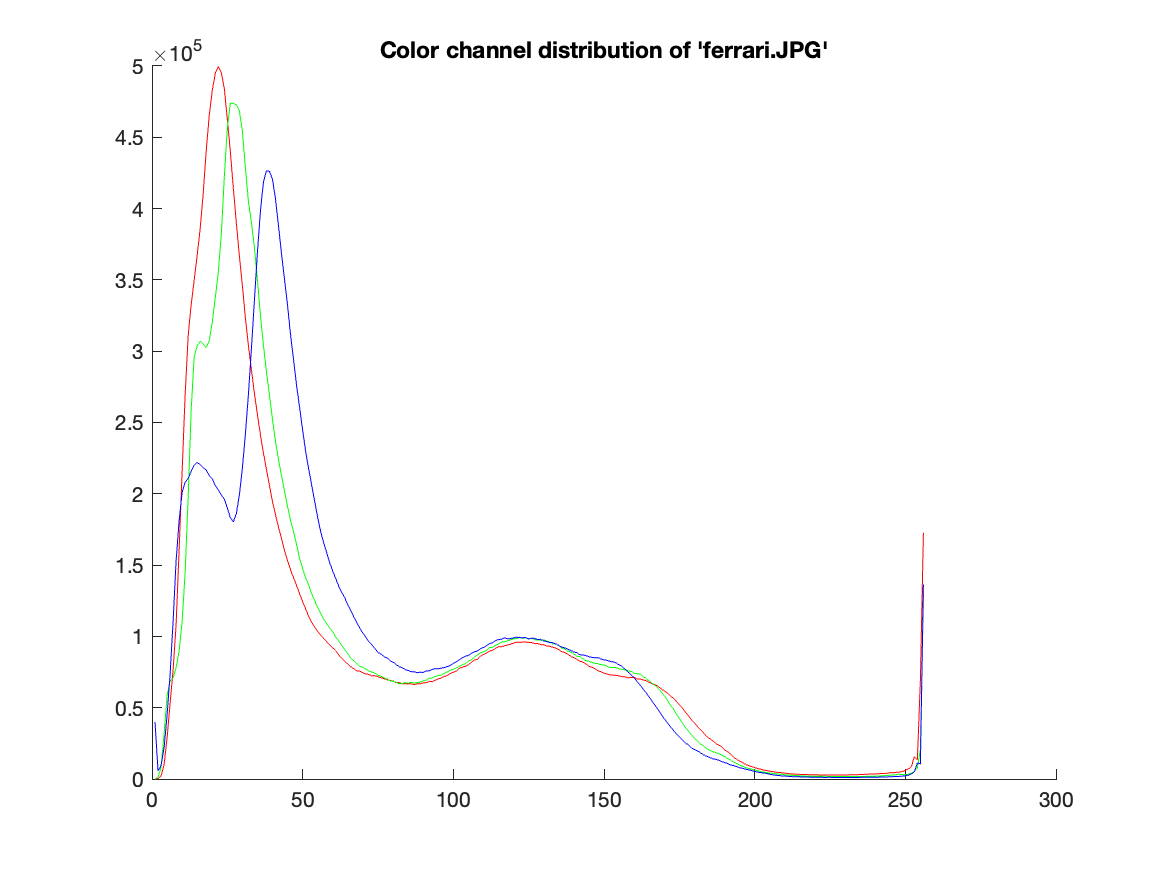
\includegraphics[width=0.5\linewidth]{fig/out/3.histogram.png}
    \caption{Color channel distribution of the image $\texttt{ferrari.JPG}$.}
\end{figure}
\subsection{Histogram Equalization [5 points + 2 Bonus]}
Histogram equalization is a tecnique used to redistribute pixel intensities in order to improve details in low-contrast regions. We compress the details of the intensity regions that do not contain much information, and we expand the details of the regions that contain more information.\\\\
% TODO: Theory questions
When handling compressed images, as intensity values are represented with less precision, equalization may result in an increase in artifacts as remapping pixel intensities may lead to rounding errors resulting in abrupt variations of intensities (i.e noise). Also regions of similar intensities may not increase in detail once histogram equalization is applied, as the slight variations in intensities (i.e details) may not be representable with a limited amount of bits.\\
The image histogram after equalization will have the regions of high densities smoothed out and enlarged, while the low density regions will get squeezed resulting in higher pixel counts. Therefore the histogram will look overall flatter.



\begin{itemize}
    \item \textbf{Global equalization}\\
    We calculate the cumulative distribution function of the images' Value channel distribution and use it to map the intensities from the old image into the new, equalized one. Results are shown in Figure \ref{fig:4.1.ferrari_globalnorm}.
    \begin{minted}[framesep=2mm, fontsize=\small]{matlab} 
function [equalized_channel, original_brightness_distribution] = global_histogram_equalization(imhsv)
    channel = imhsv(:,:,3);
    % Cumulative distribution function of the image histogram
    [original_brightness_distribution, ~ ] = imhist(channel);
    cdf = cumsum(original_brightness_distribution);
    cdf = cdf / cdf(end);
    % Apply the transformation
    equalized_channel = cdf(round(channel*255+1));
end
    \end{minted}
    \item \textbf{Local equalization}\\
    We subdivide the frame into tiles and we equalize them separately using global equalization. Results are shown in Figure \ref{fig:4.2.ferrari_localnorm}.
    \begin{minted}[framesep=2mm, fontsize=\small]{matlab} 
function [imhsv_equalized] = local_histogram_equalization(imhsv, TILENO)
    imhsv_equalized = imhsv;
    im_size = size(imhsv_equalized);
    tile_size = floor((im_size(1:2)/TILENO));
    for row = 0:TILENO-1
        for col = 0:TILENO-1
            imageUB = round(([row col].*tile_size)) + 1;
            imageLB = round(([row col].*tile_size) + tile_size);
            tile = imhsv_equalized(imageUB(1):imageLB(1),imageUB(2):imageLB(2),:);
            [equalized_tile, ~ ] = global_histogram_equalization(tile);
            imhsv_equalized(imageUB(1):imageLB(1),imageUB(2):imageLB(2),3) = equalized_tile;
        end
    end
end
    \end{minted}
    \item \textbf{Locally adaptive equalization}\\
    We equalize each pixel by using a moving window that has the pixel at its center. We run the standard global equalization on the window and we apply the transformation to the pixel. Results are shown in Figure \ref{fig:4.3.ferrari_adaptivenorm}.
    \begin{minted}[framesep=2mm, fontsize=\small]{matlab} 
function [imhsv_equalized] = locally_adaptive_histogram_equalization(imhsv, TILESIZE)
    imhsv_equalized = imhsv;
    im_size = size(imhsv_equalized);
    for y = 1:im_size(1)
        for x = 1:im_size(2)
            % Coordinates of the top-left corner of the moving window.
            imageUB = round(max([[y x] - (TILESIZE/2); 1 1]));
            % Coordinates of the bottom-right corner of the moving window.
            imageLB = round(min([[y x] + (TILESIZE/2); im_size(1:2)]));
            tile = imhsv_equalized(imageUB(1):imageLB(1), imageUB(2):imageLB(2),:);
            [equalized_tile, ~ ] = global_histogram_equalization(tile);
            imhsv_equalized(y,x,3) = equalized_tile(y-imageUB(1)+1, x-imageUB(2)+1);
        end
    end
end
    \end{minted}
\begin{minted}[framesep=2mm, fontsize=\small]{matlab} 

\end{minted}
\end{itemize}
\begin{figure}[h!]
    \begin{subfigure}{0.24\textwidth}
        \centering
        \includegraphics[width=\textwidth]{fig/out/4.1.ferrari.png}
        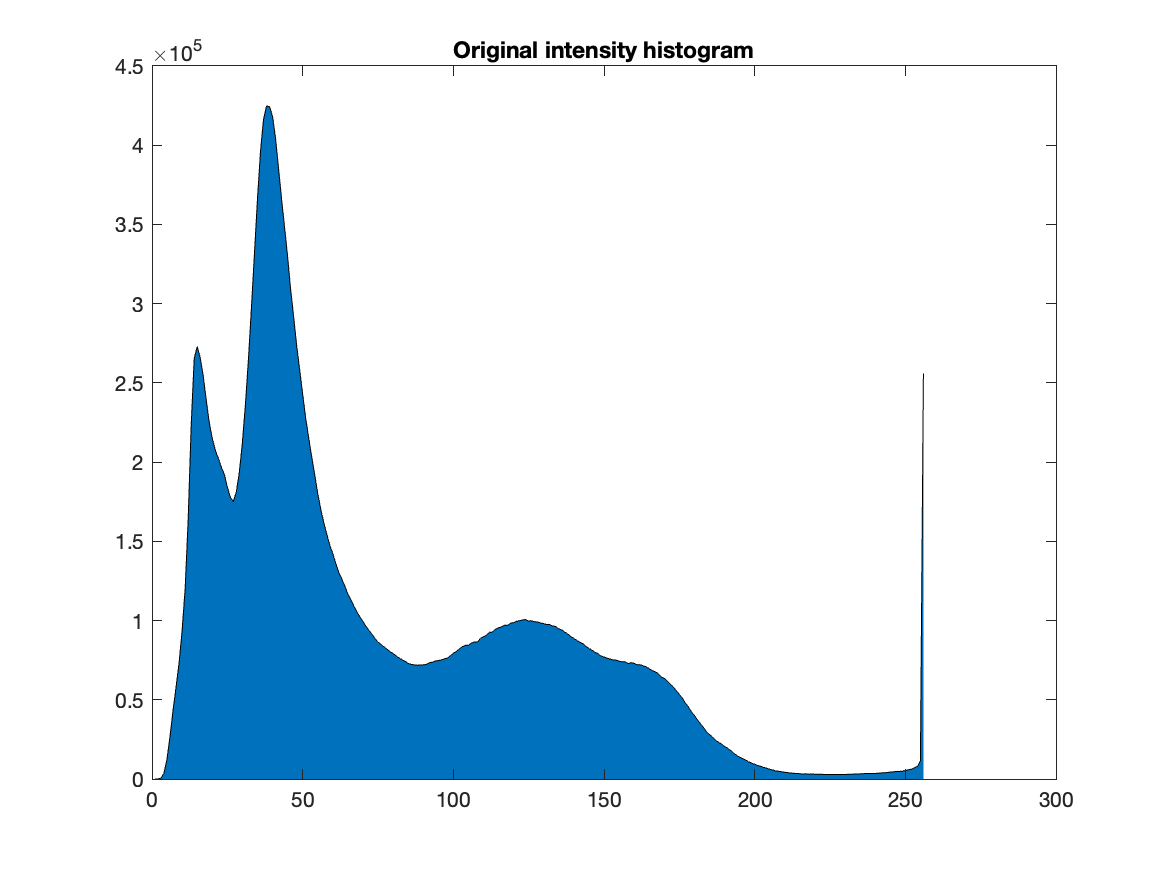
\includegraphics[width=\textwidth]{fig/out/4.1.ferrari_hist.png}
        \caption{Original image.}
    \end{subfigure}
    \begin{subfigure}{0.24\textwidth}
        \centering
        \includegraphics[width=\textwidth]{fig/out/4.1.ferrari_globalnorm.png}
        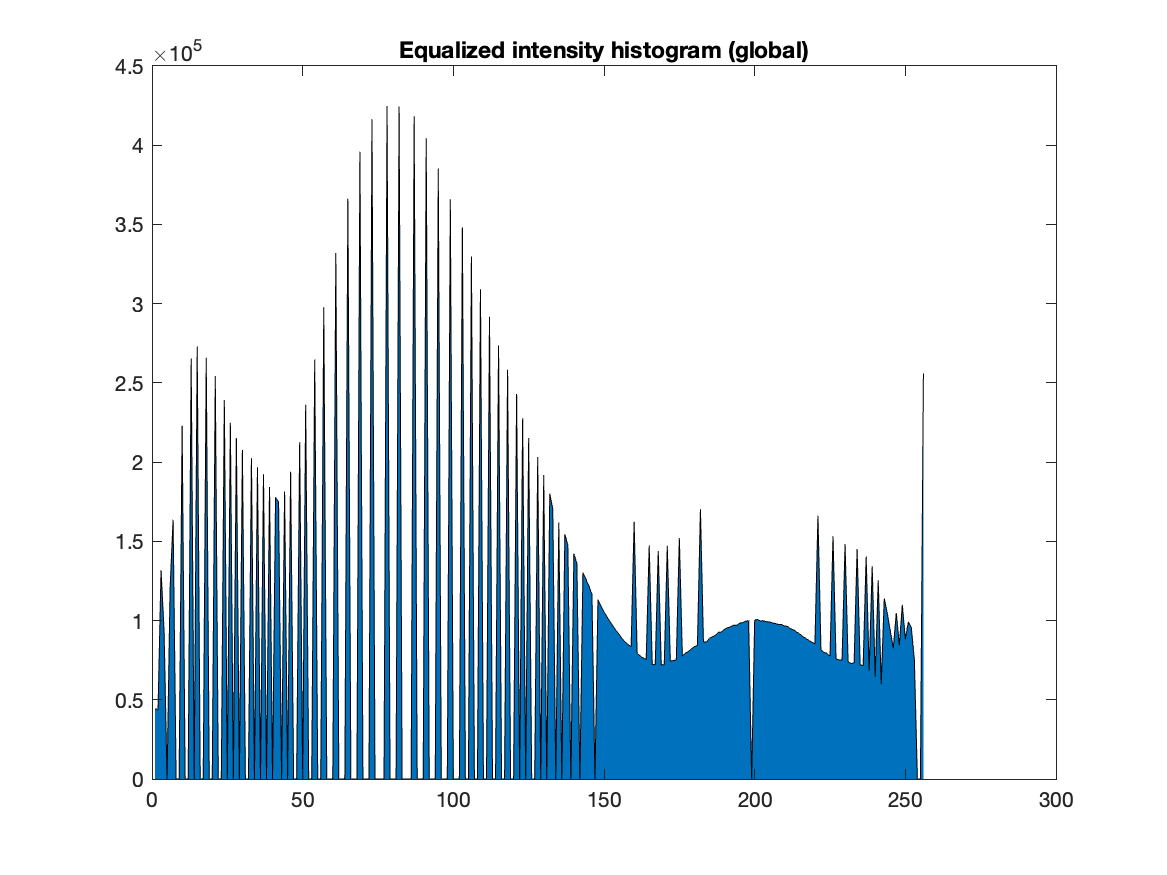
\includegraphics[width=\textwidth]{fig/out/4.1.ferrari_globalnorm_hist.png}
        \caption{Global eq.}
        \label{fig:4.1.ferrari_globalnorm}
    \end{subfigure}
    \begin{subfigure}{0.24\textwidth}
        \centering
        \includegraphics[width=\textwidth]{fig/out/4.2.ferrari_localnorm.png}
        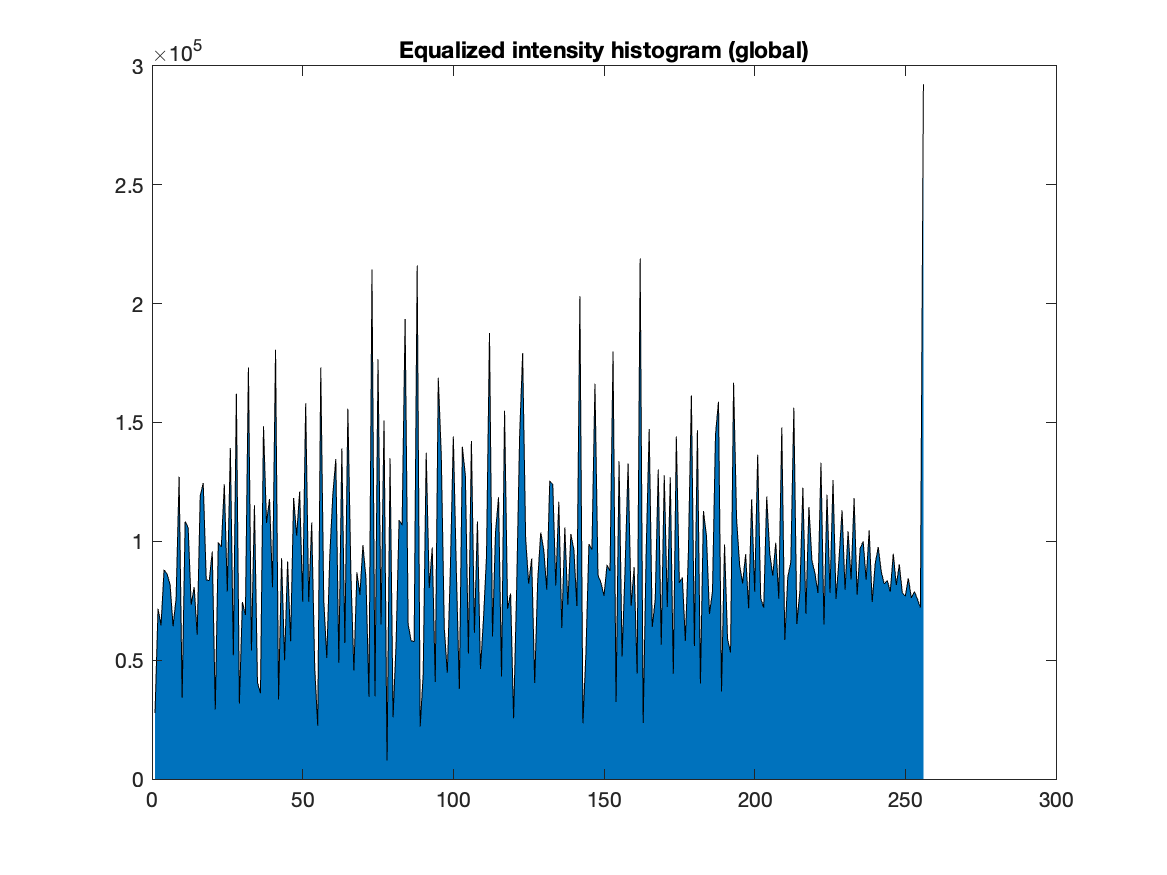
\includegraphics[width=\textwidth]{fig/out/4.2.ferrari_localnorm_hist.png}
        \caption{Local eq. (4x4 tiles)}
        \label{fig:4.2.ferrari_localnorm}
    \end{subfigure}
    \begin{subfigure}{0.24\textwidth}
        \centering
        \includegraphics[width=\textwidth]{fig/out/4.3.ferrari_locallyadaptivenorm.png}
        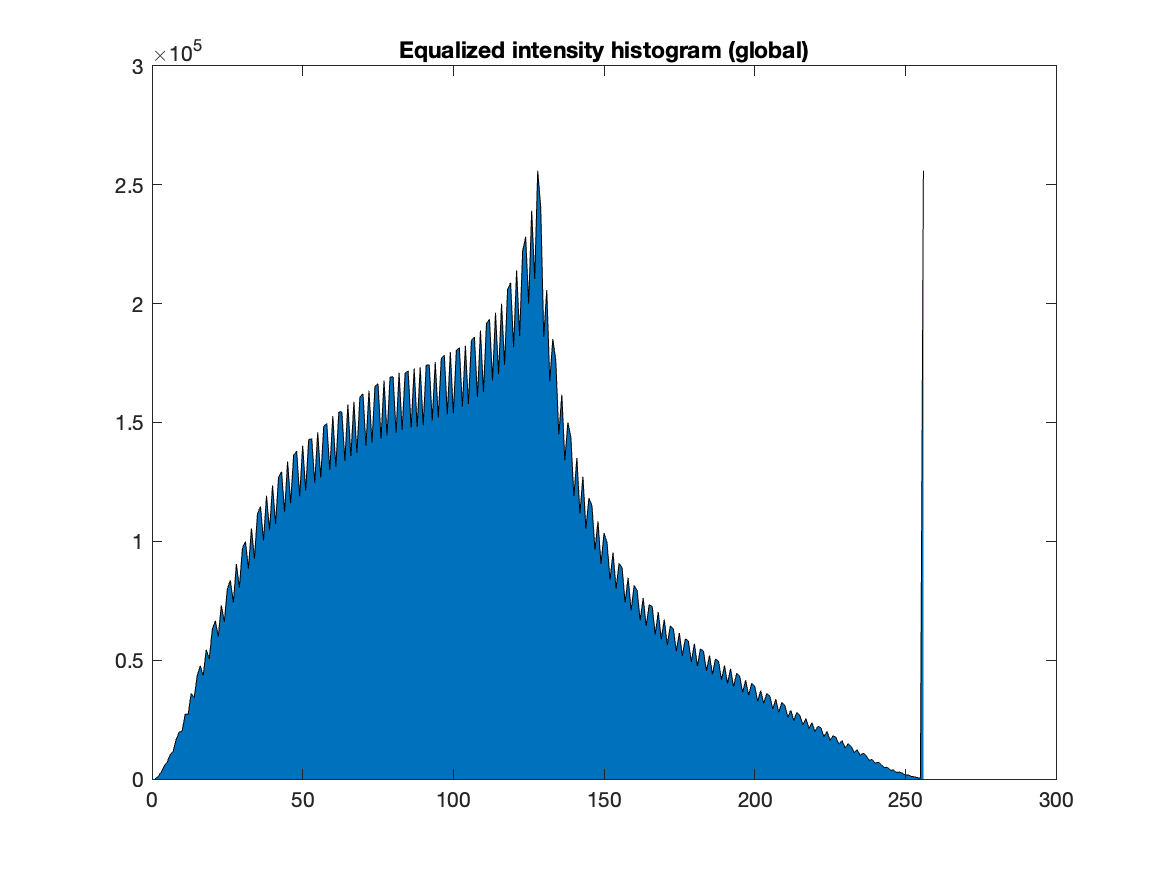
\includegraphics[width=\textwidth]{fig/out/4.3.ferrari_locallyadaptivenorm_hist.png}
        \caption{Locally adaptive eq.}
        \label{fig:4.3.ferrari_adaptivenorm}
    \end{subfigure}

    \caption{Comparison of different histogram equalization techniques.}
\end{figure}
\subsection{Manual histogram equalization [2 points]}
A cumulative distribution function (CDF) of the image histogram tells us the probability that a pixel has an intensity less or equal to a certain value. As we can see from the image, the CDF grows in high-density regions and stays almost the same in low-density regions. 
\begin{figure}
    \centering
    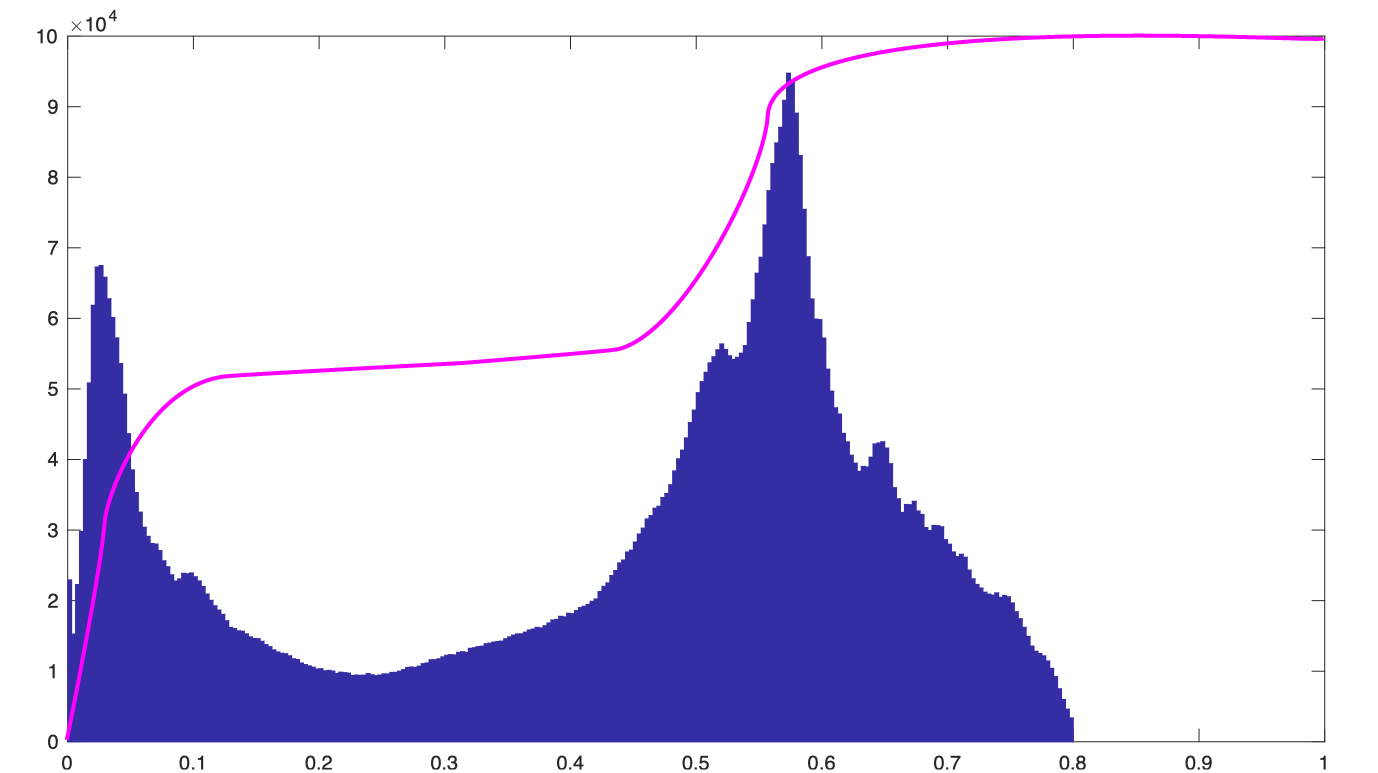
\includegraphics[width=0.3\textwidth]{fig/1.5.hist.png}
    \caption{Original image.}
\end{figure}

\subsection{Thresholding \& matting [4 points]}
The chroma key implementation is rather straightforward. We let the user choose the pixel color that will be used when deriving the mask to isolate the cat subject from the background. Since the green background is not homogeneous, we define a set of threshold values for each color channel in order to take into account the variability of the background. We then apply the mask to the original image and replace the pixels that are not masked with the background image. The results are shown in Figure \ref{fig:6.comp}. 
\begin{figure}[h!]
    \begin{center}
    \begin{subfigure}{0.22\textwidth}
        \centering
        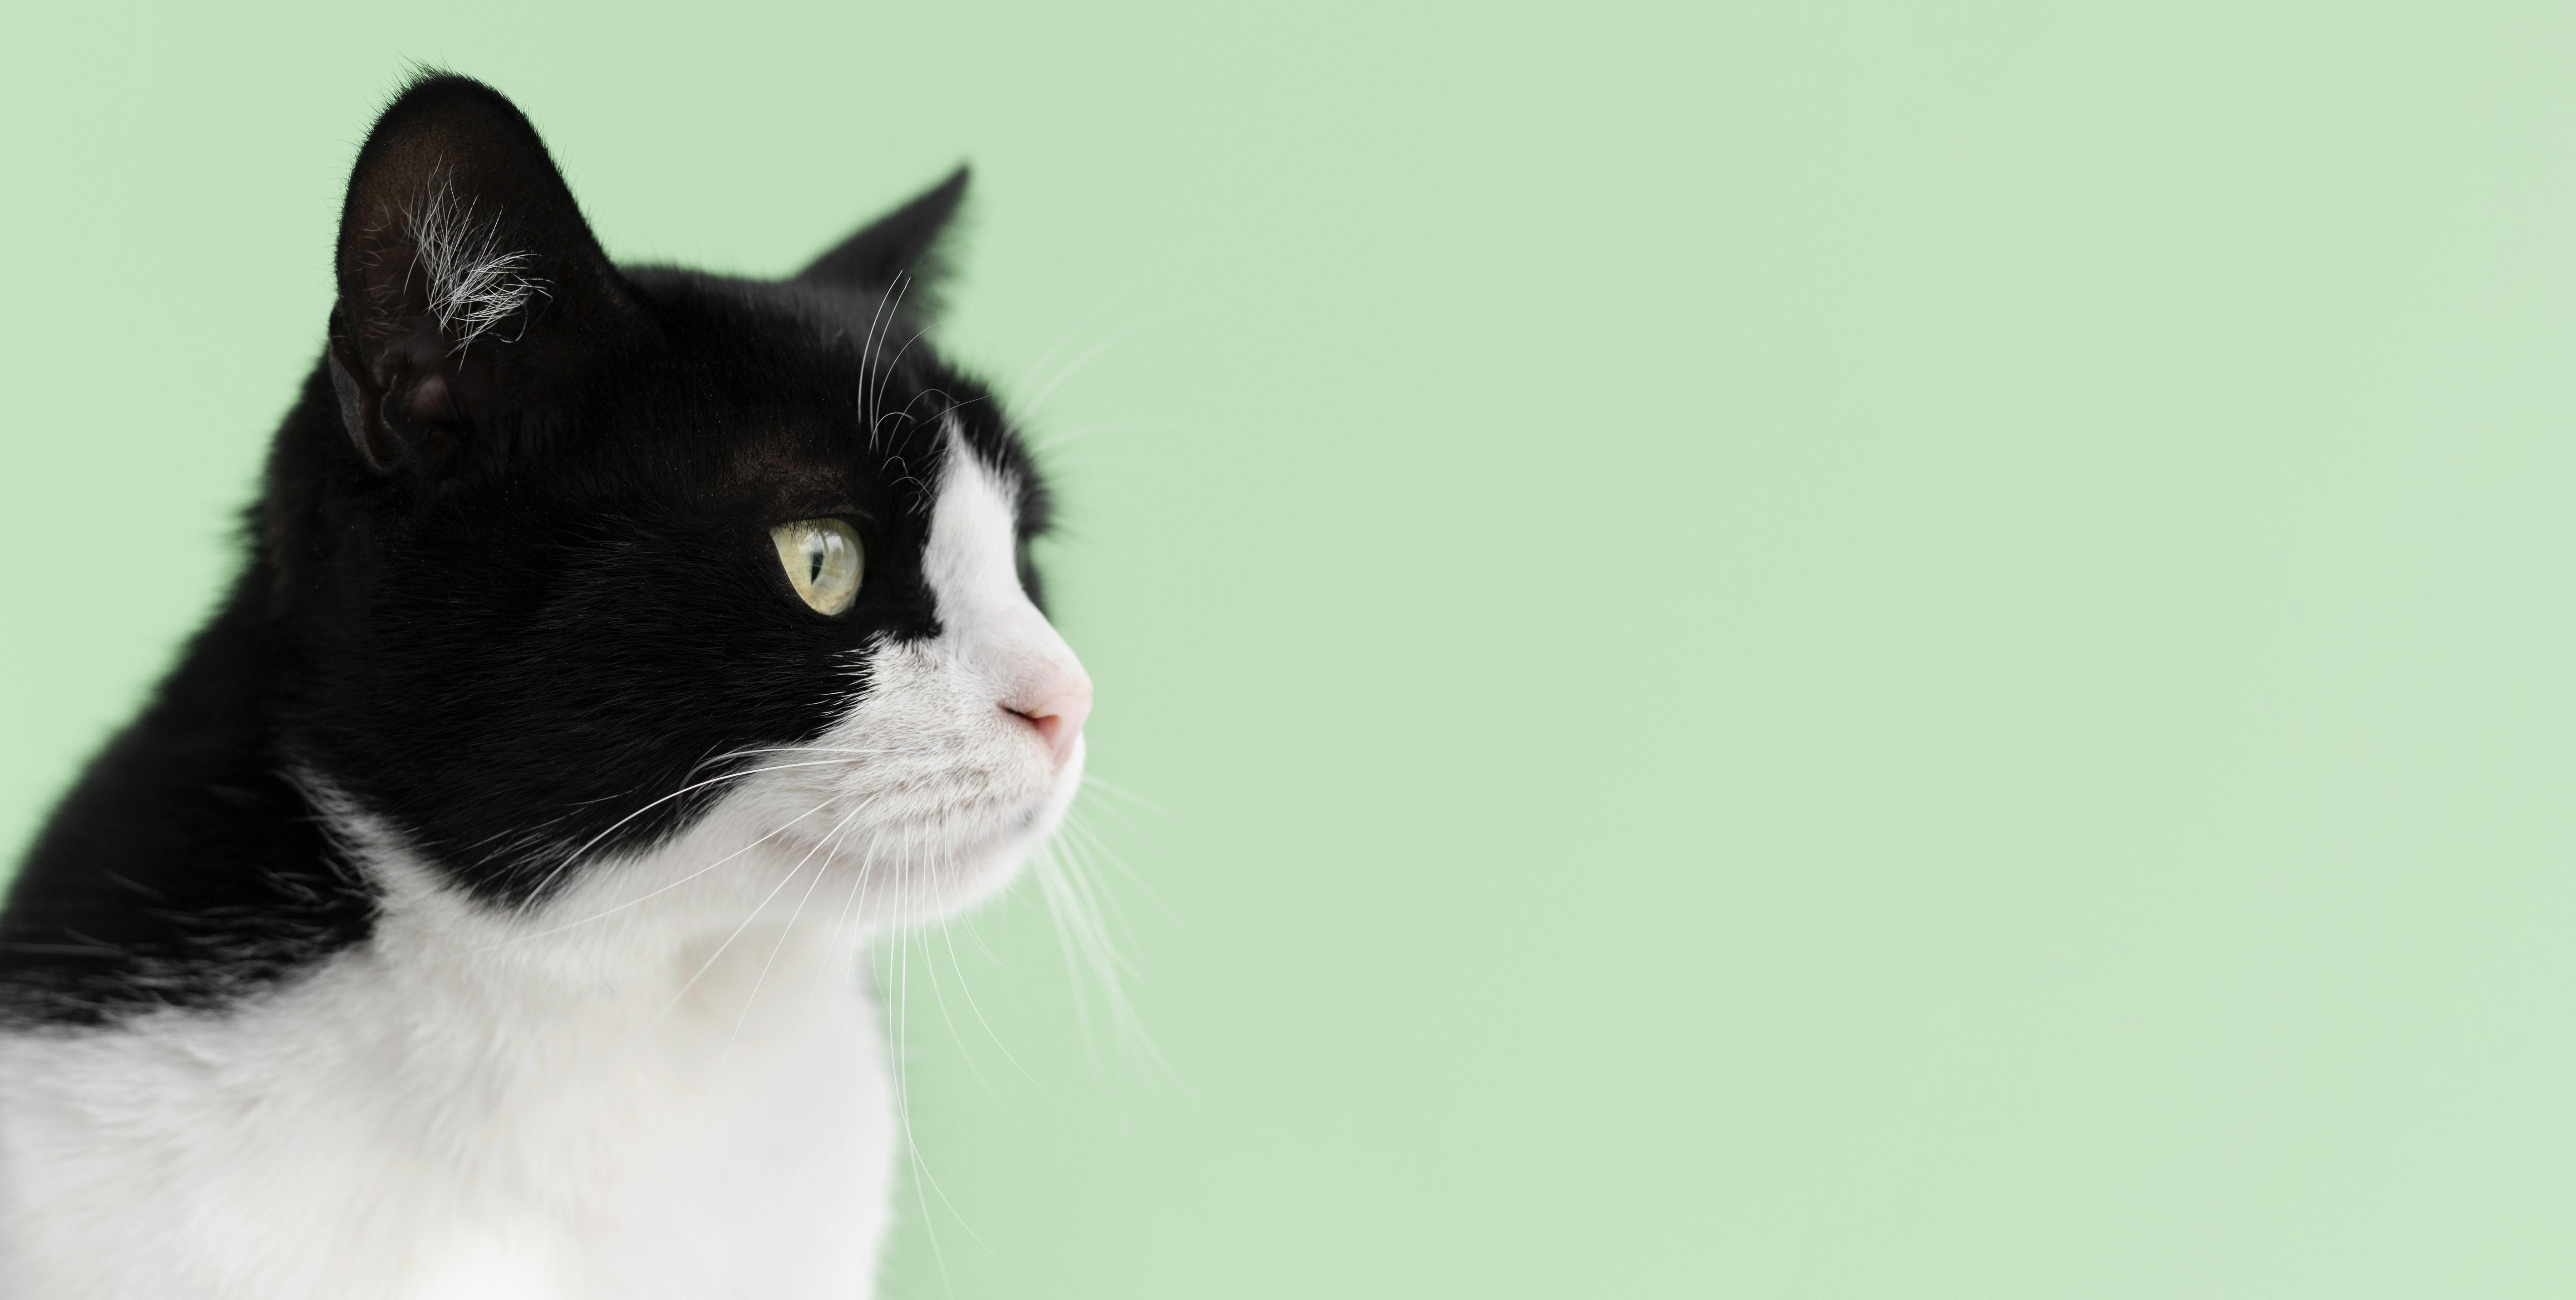
\includegraphics[width=\textwidth]{fig/out/6.cat.jpg}
        \caption{Original image.}
    \end{subfigure}
    \begin{subfigure}{0.22\textwidth}
        \centering
        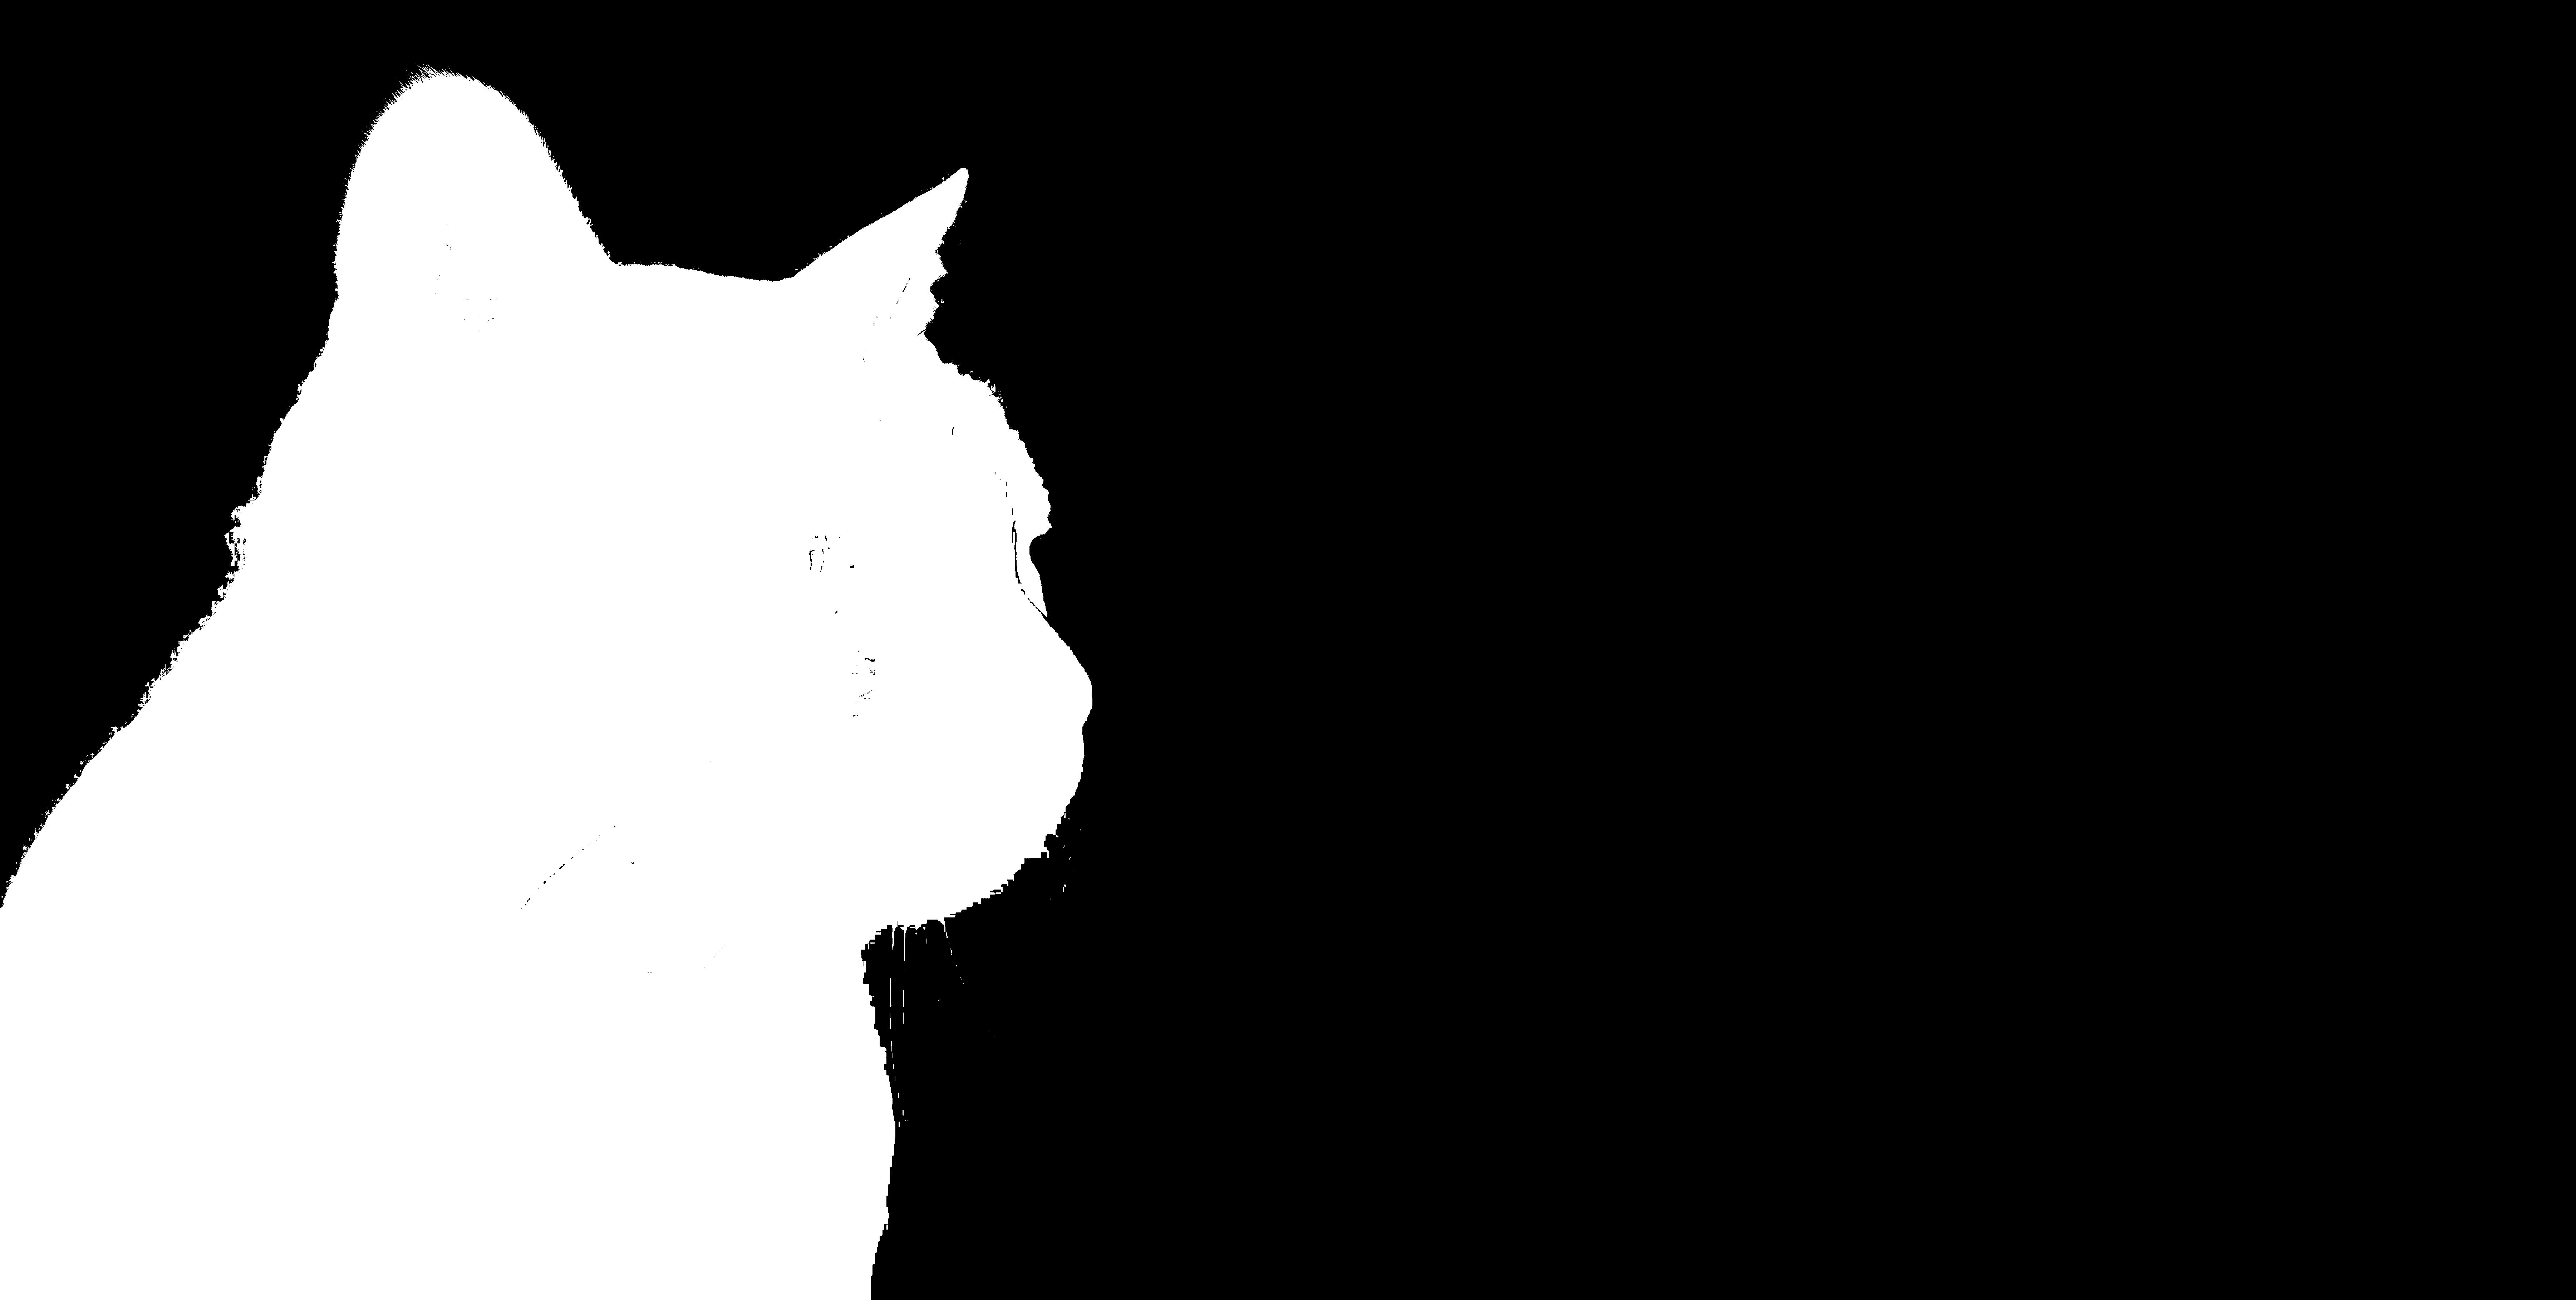
\includegraphics[width=\textwidth]{fig/out/6.mask.jpg}
        \caption{Chroma Key mask.}
    \end{subfigure}
    \begin{subfigure}{0.22\textwidth}
        \centering
        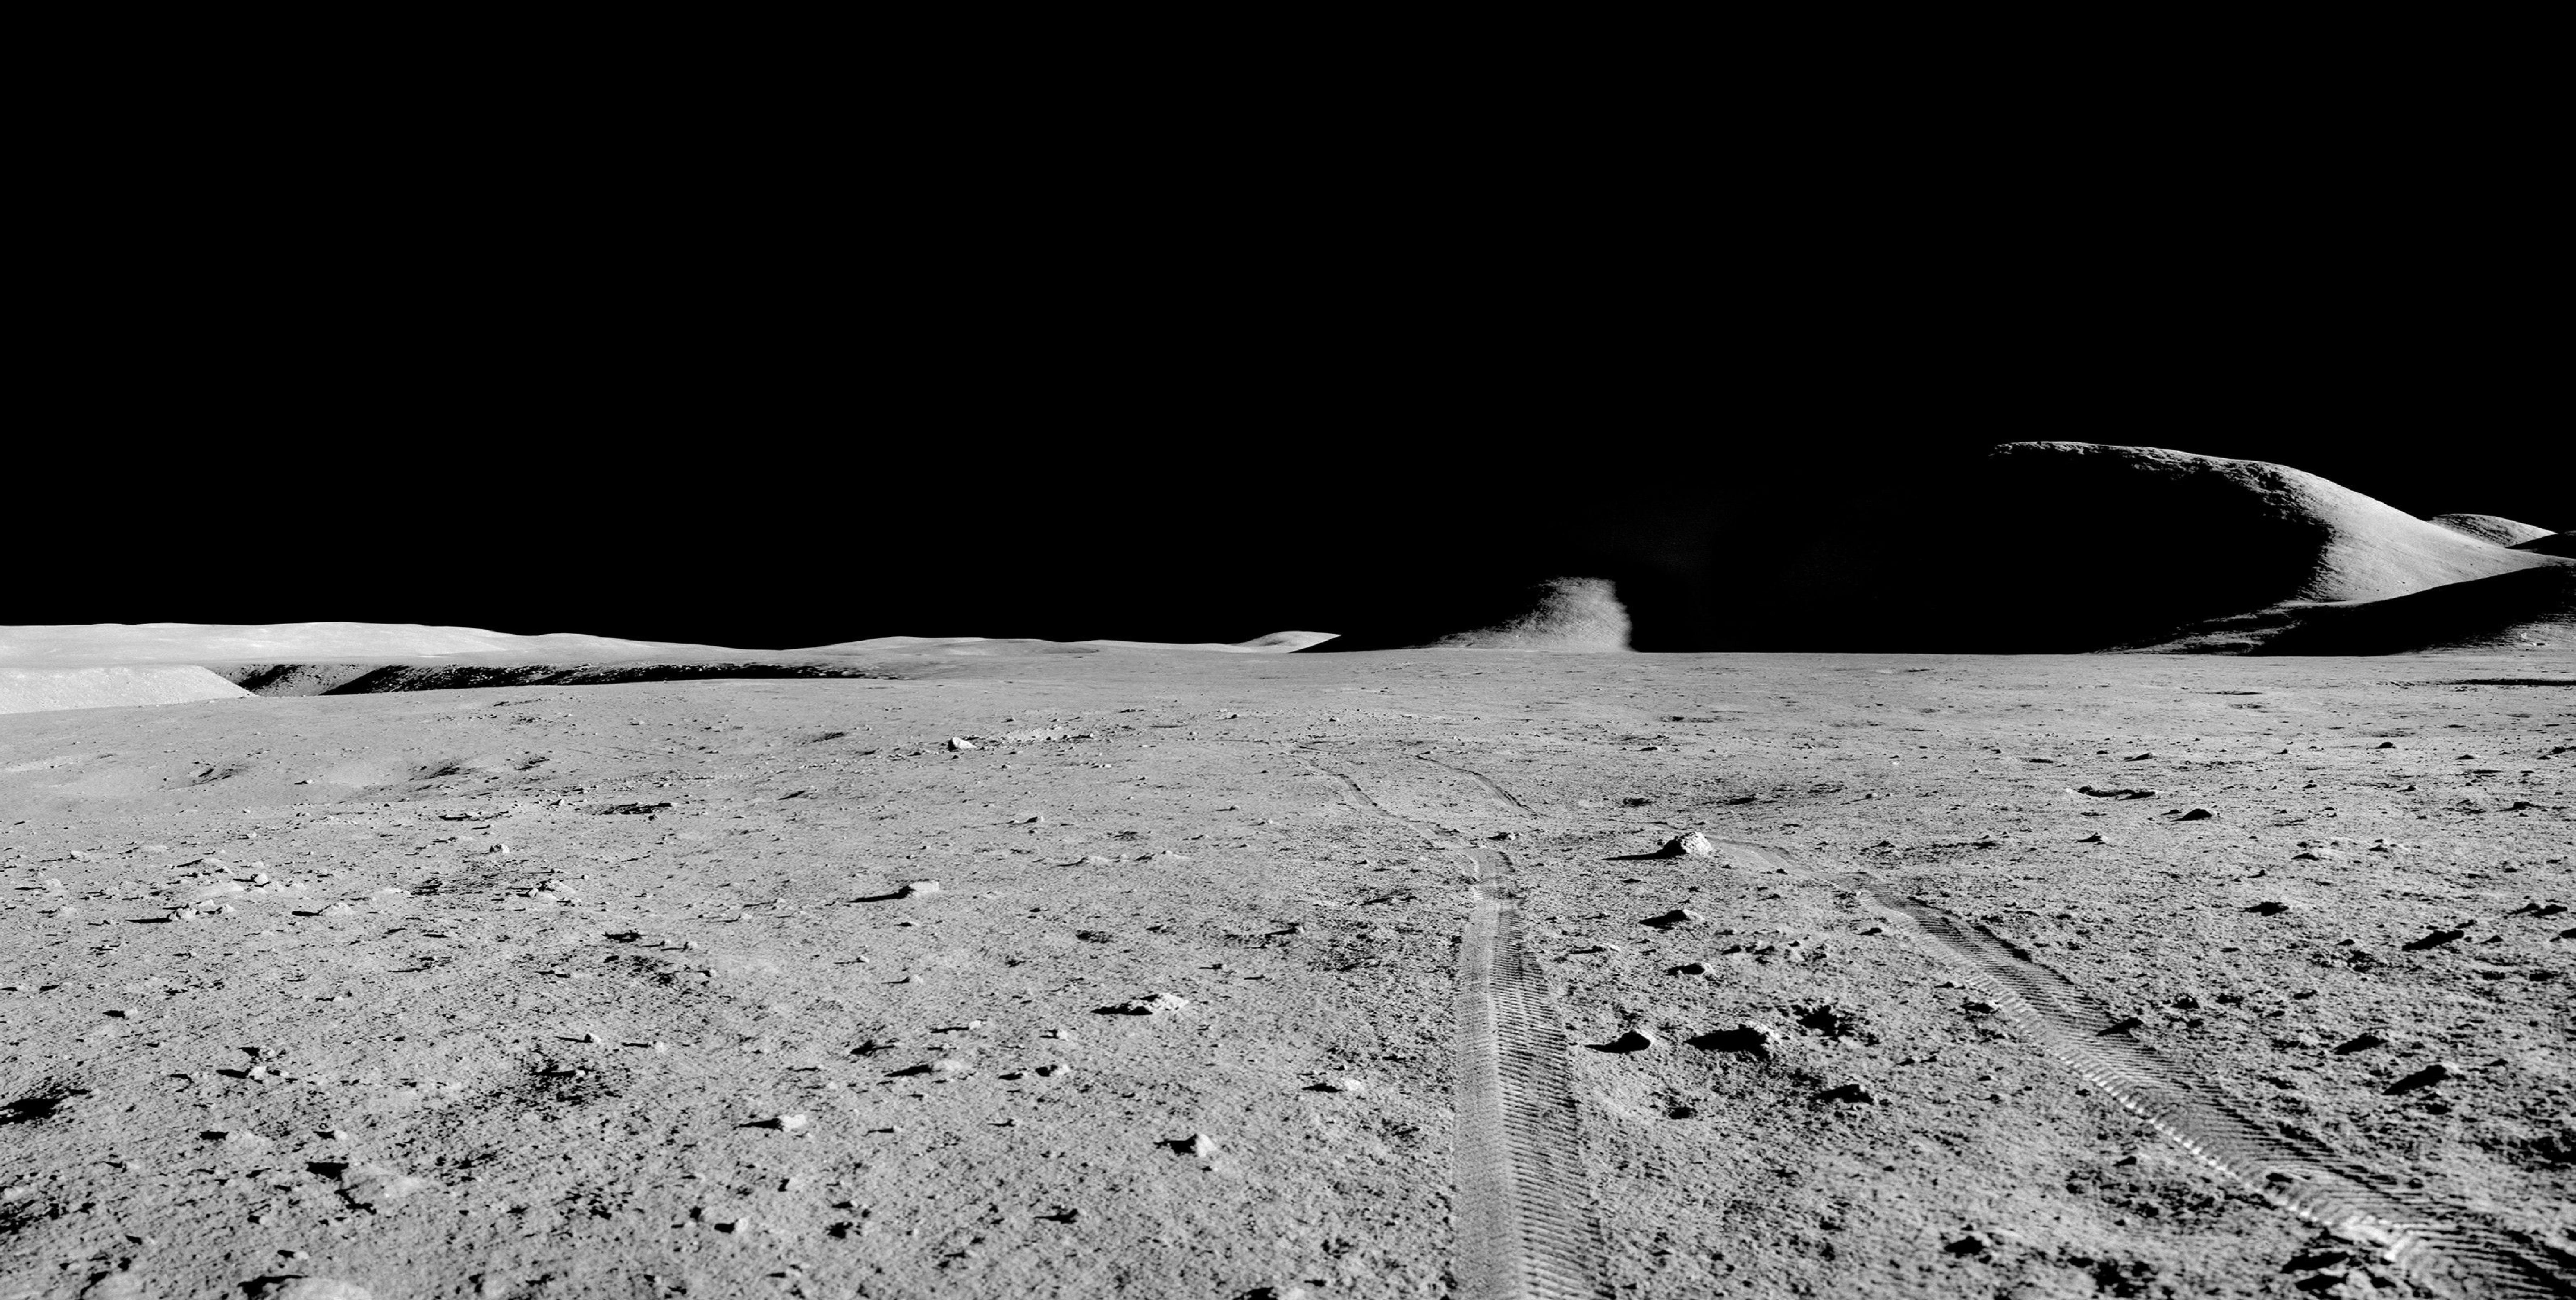
\includegraphics[width=\textwidth]{fig/out/6.spacebg.jpg}
        \caption{Background image.}
    \end{subfigure}

    \begin{subfigure}{.67\textwidth}
        \centering
        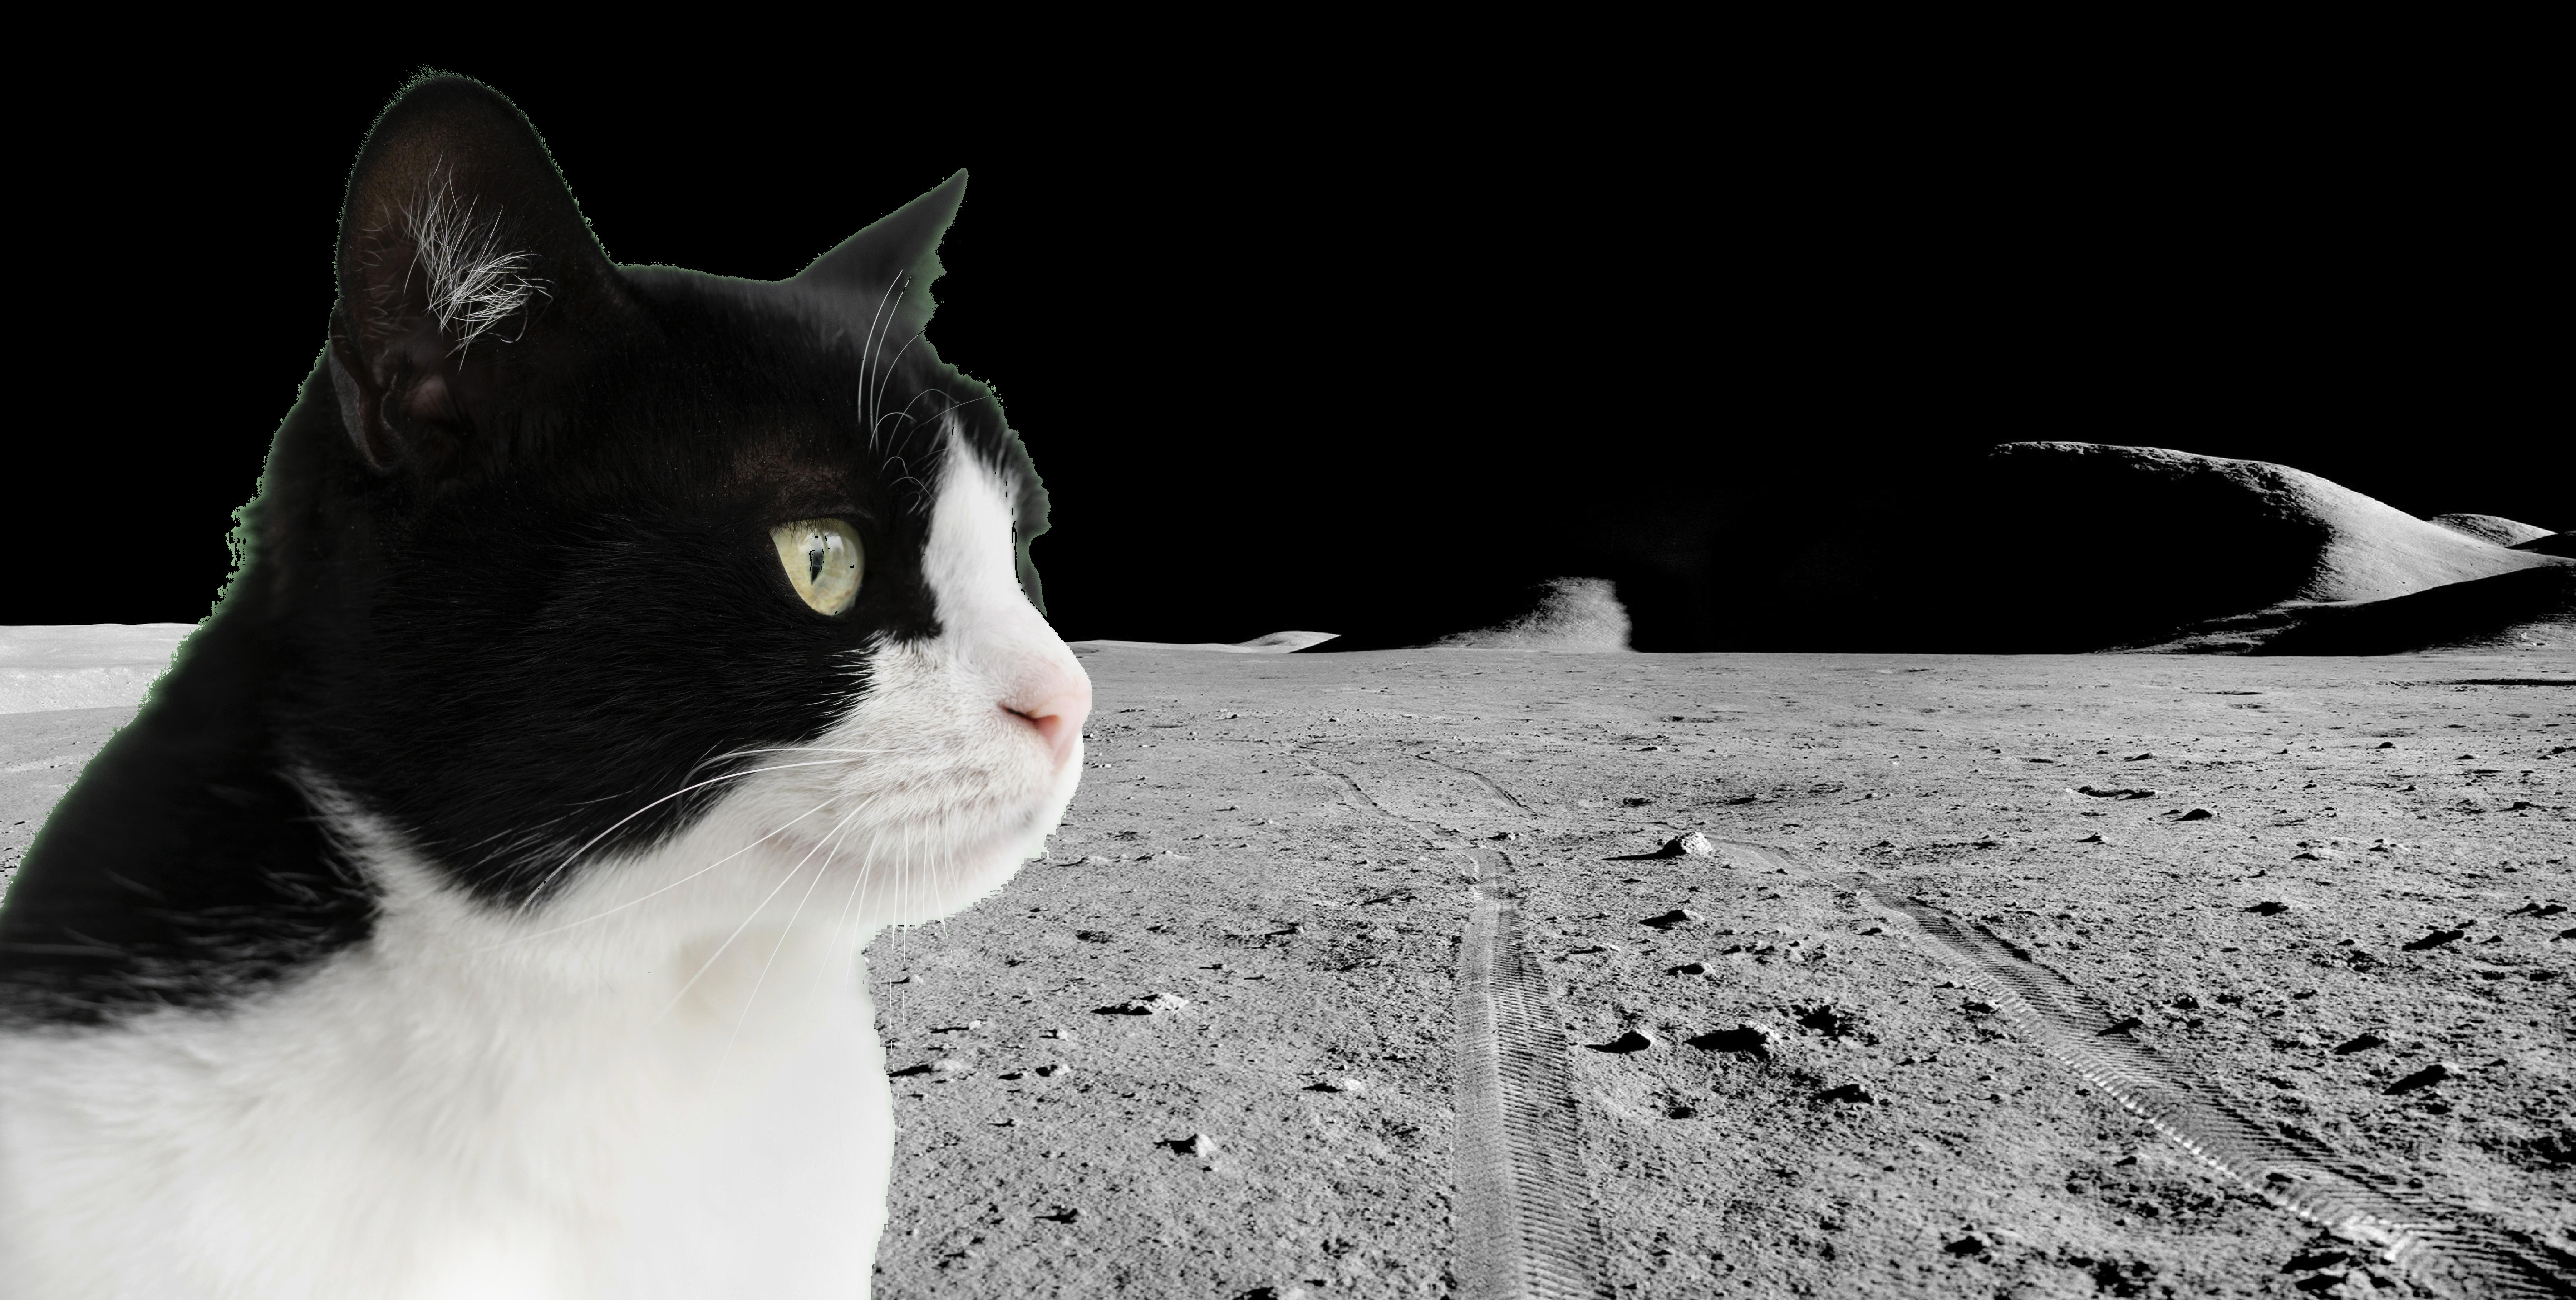
\includegraphics[width=\textwidth]{fig/out/6.comp.jpg}
        \caption{Composited result image.}
        \label{fig:6.comp}
    \end{subfigure}
\end{center}
    \caption{Chroma key compositing}
\end{figure}

\begin{figure}[h!]
    \begin{minted}[ frame=lines, framesep=2mm, linenos, fontsize=\small ]{matlab} 
%...
% Lets the user select a pixel in the image to key out.
figure(); imshow(im);
coords = int32(ginput(1));
px_hsv = imhsv(coords(2), coords(1), 1:3);

%  Each channel may deviate of these amounts from the selected pixel.
hue_deviation = 0.05;
saturation_deviation = 0.1; % += 10% saturation
brightness_deviation = 0.4; % += 40% darker/lighter

% Creates the mask for each pixel whose channels are within the deviations
mask = ~(abs(imhsv(:,:,1) - px_hsv(1)) <= hue_deviation & ...
            abs(imhsv(:,:,2) - px_hsv(2)) <= saturation_deviation & ...
            abs(imhsv(:,:,3) - px_hsv(3)) <= brightness_deviation);
im_mask = comp(ones(size(im)), mask,zeros(size(im)));
im_comp = comp(im,mask,im_spacebg);

function res = comp(a,mask,b)
    % Masks image 'a' on top of image 'b'
    res = a.*mask + b.*(~mask);
end
    \end{minted}
\caption{Matlab code performing background replacement on image \texttt{cat.jpg}.}
\end{figure}

\subsection{How many bits is enough [2 points]}
We know that:
$$\frac{I_{max}}{I_{min}} = (1+k)^{N-1}$$
Where $I_{max}$ is the maximum intensity value, $I_{min}$ is the minimum intensity value, $k$ is the Weber Constant and $N$ the amount of bits used for encoding.\\
We are given the luminance range of the display and the Weber Constant:
$$I_{min} = 0.5, I_{max} = 1000, k = 0.01$$
Let us substitute and solve for $N$:
\begin{align*}
    \frac{1000}{\frac{1}{2}} &= (1+0.01)^{N-1}\\
    \log_{\frac{101}{100}}(2000) &= N-1\\
    763.88 &= N - 1\\
    N &\approx 764.88 = 765
\end{align*}
So we need to represent $765$ different values. $2^{10} = 1024$, so we need 10 bits to represent the full range of luminance values.
\section{Bonus: use your own pictures [3 points]}
I took multiple pictures of myself in different poses in my hallway. I took a cleanplate picture of my hallway and used it to compute the masks for all the other pictures. Once I had all the masks, I composited every masked picture on top of the cleanplate image. The result is shown in Figure \ref{fig:8.mourning}. Additionally I made use of function \mintinline{matlab}{medfilt2}, to denoise the masks using median filtering\footnote{Median Filtering: The median filter is a non-linear digital filtering technique, often used to remove noise from an image or signal. Such noise reduction is a typical pre-processing step to improve the results of later processing (for example, edge detection on an image). [Source \href{https://en.wikipedia.org/wiki/Median_filter}{wikipedia.org} ]}. \\Please note that the pictures were taken in challenging lighting conditions, so the results are not perfect. Improving the masking would require more time and effort in tweaking the parameters, but I think the results are still acceptable.
\begin{figure}[h!]
    \centering
    \begin{subfigure}{.69\textwidth}
        \centering
        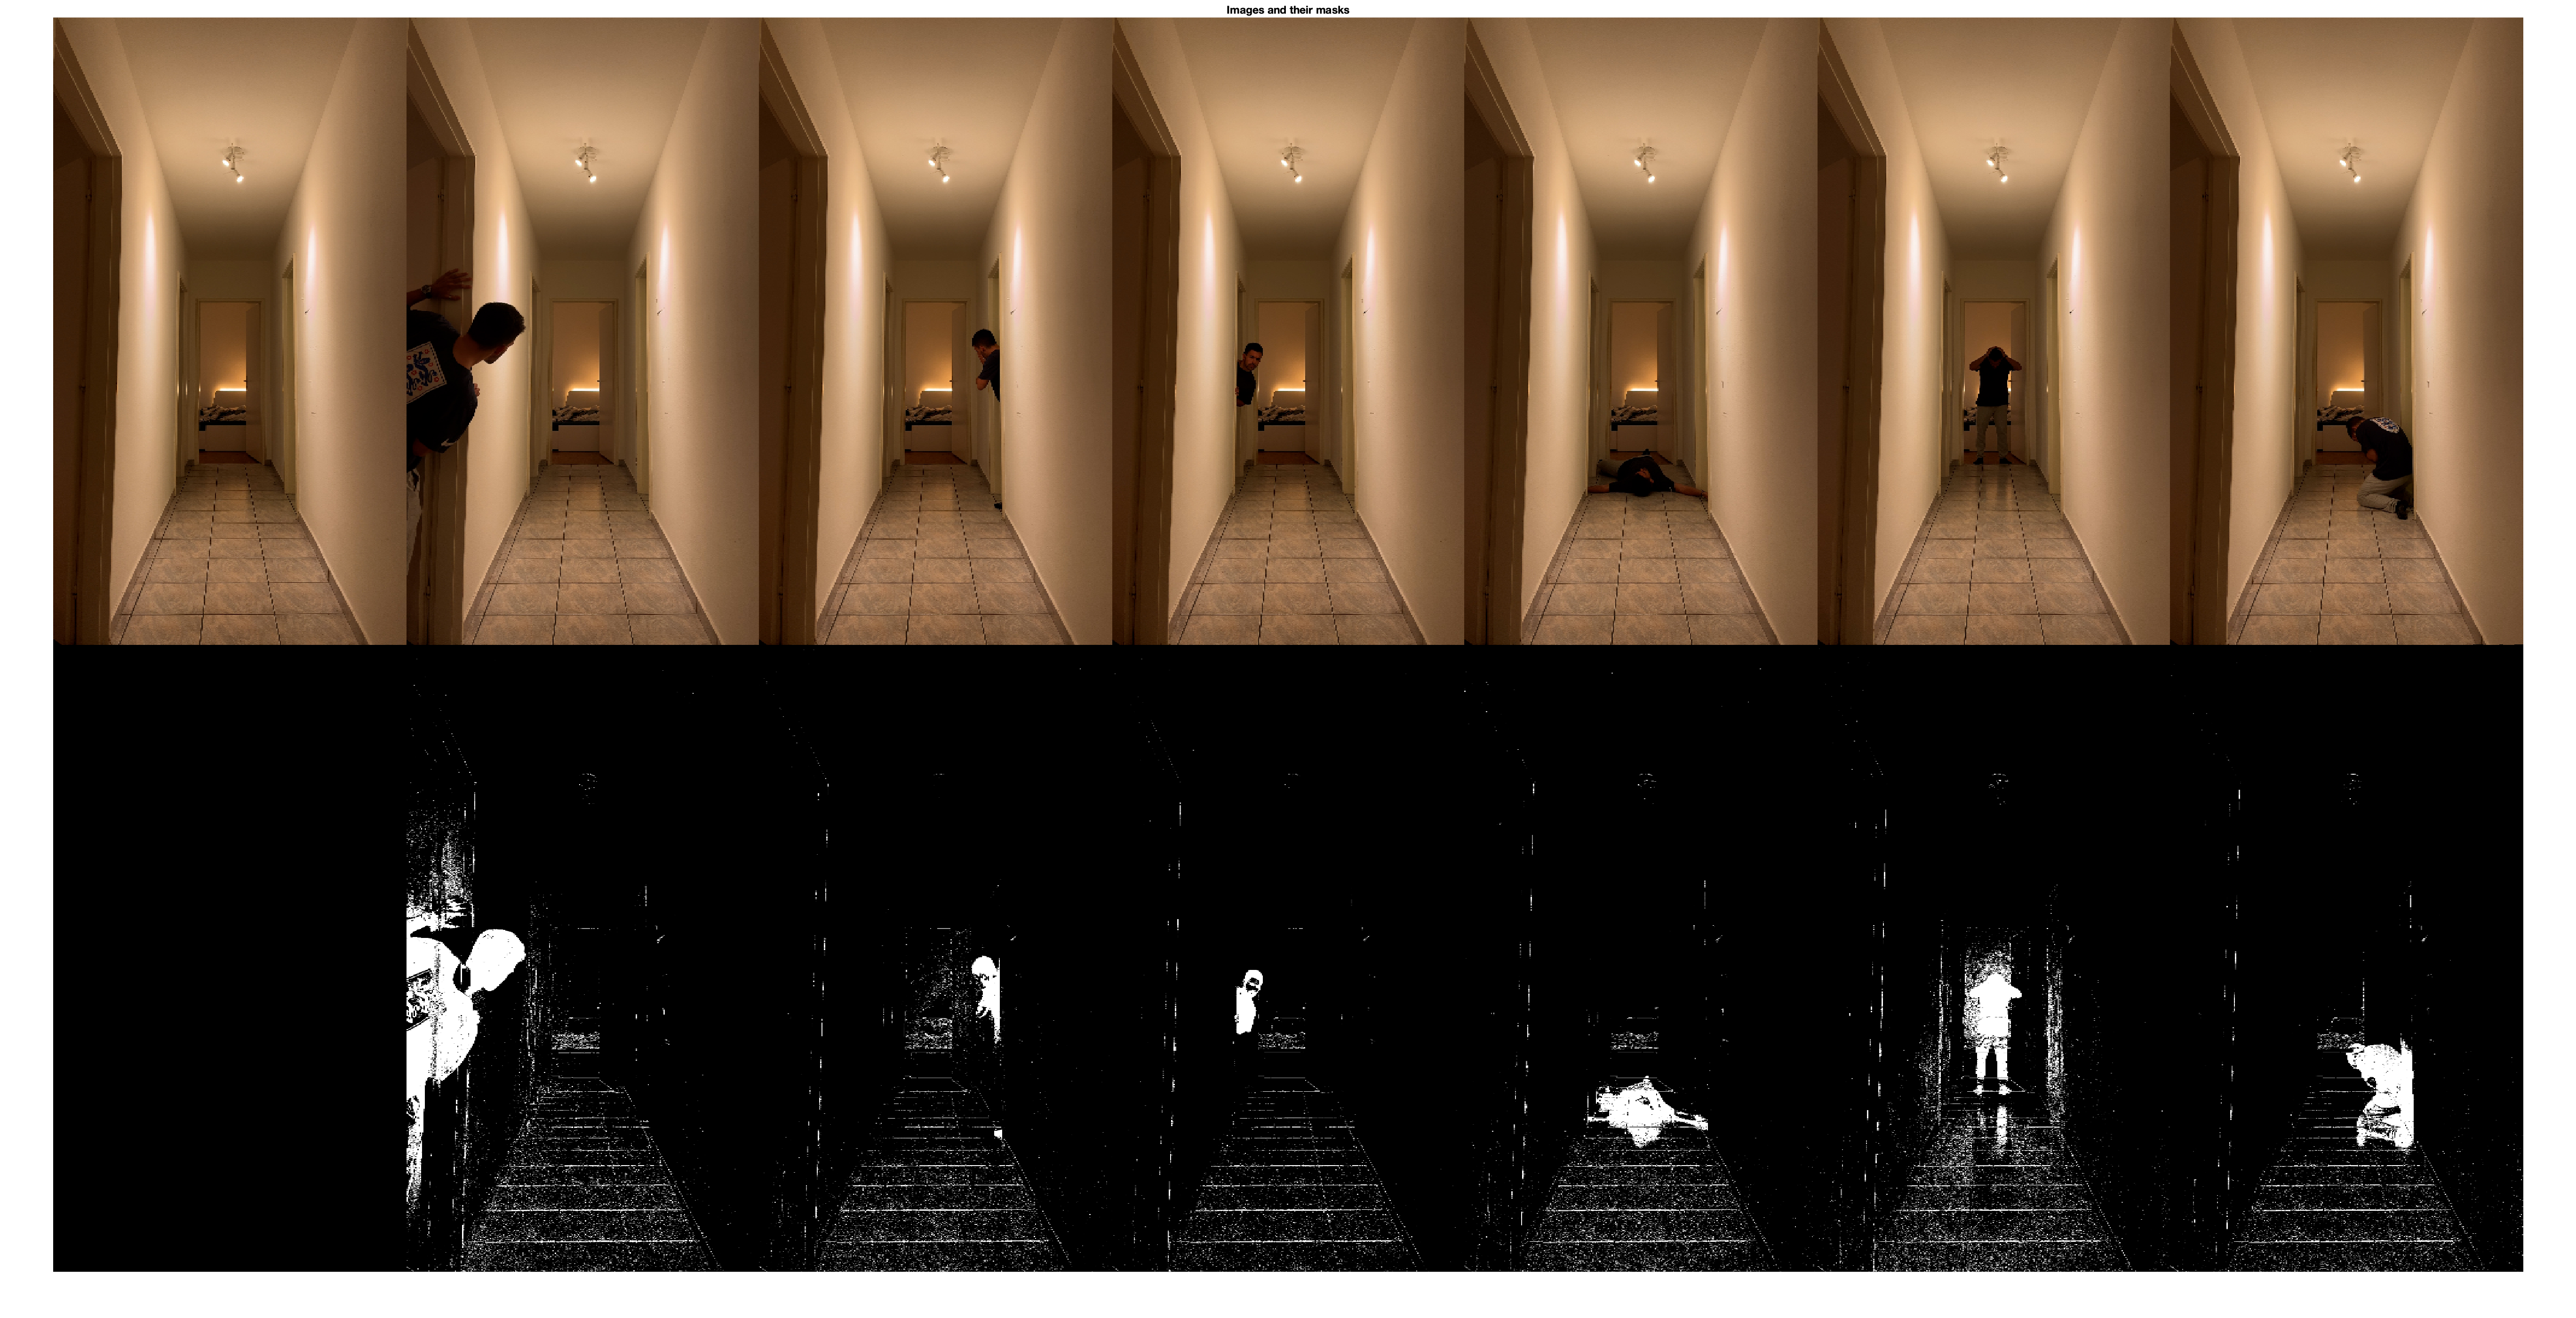
\includegraphics[width=\textwidth]{fig/out/8.images_masks.png}
        \caption{Individual pictures and relative masks.}
    \end{subfigure}
    \begin{subfigure}{0.3\textwidth}
        \centering
        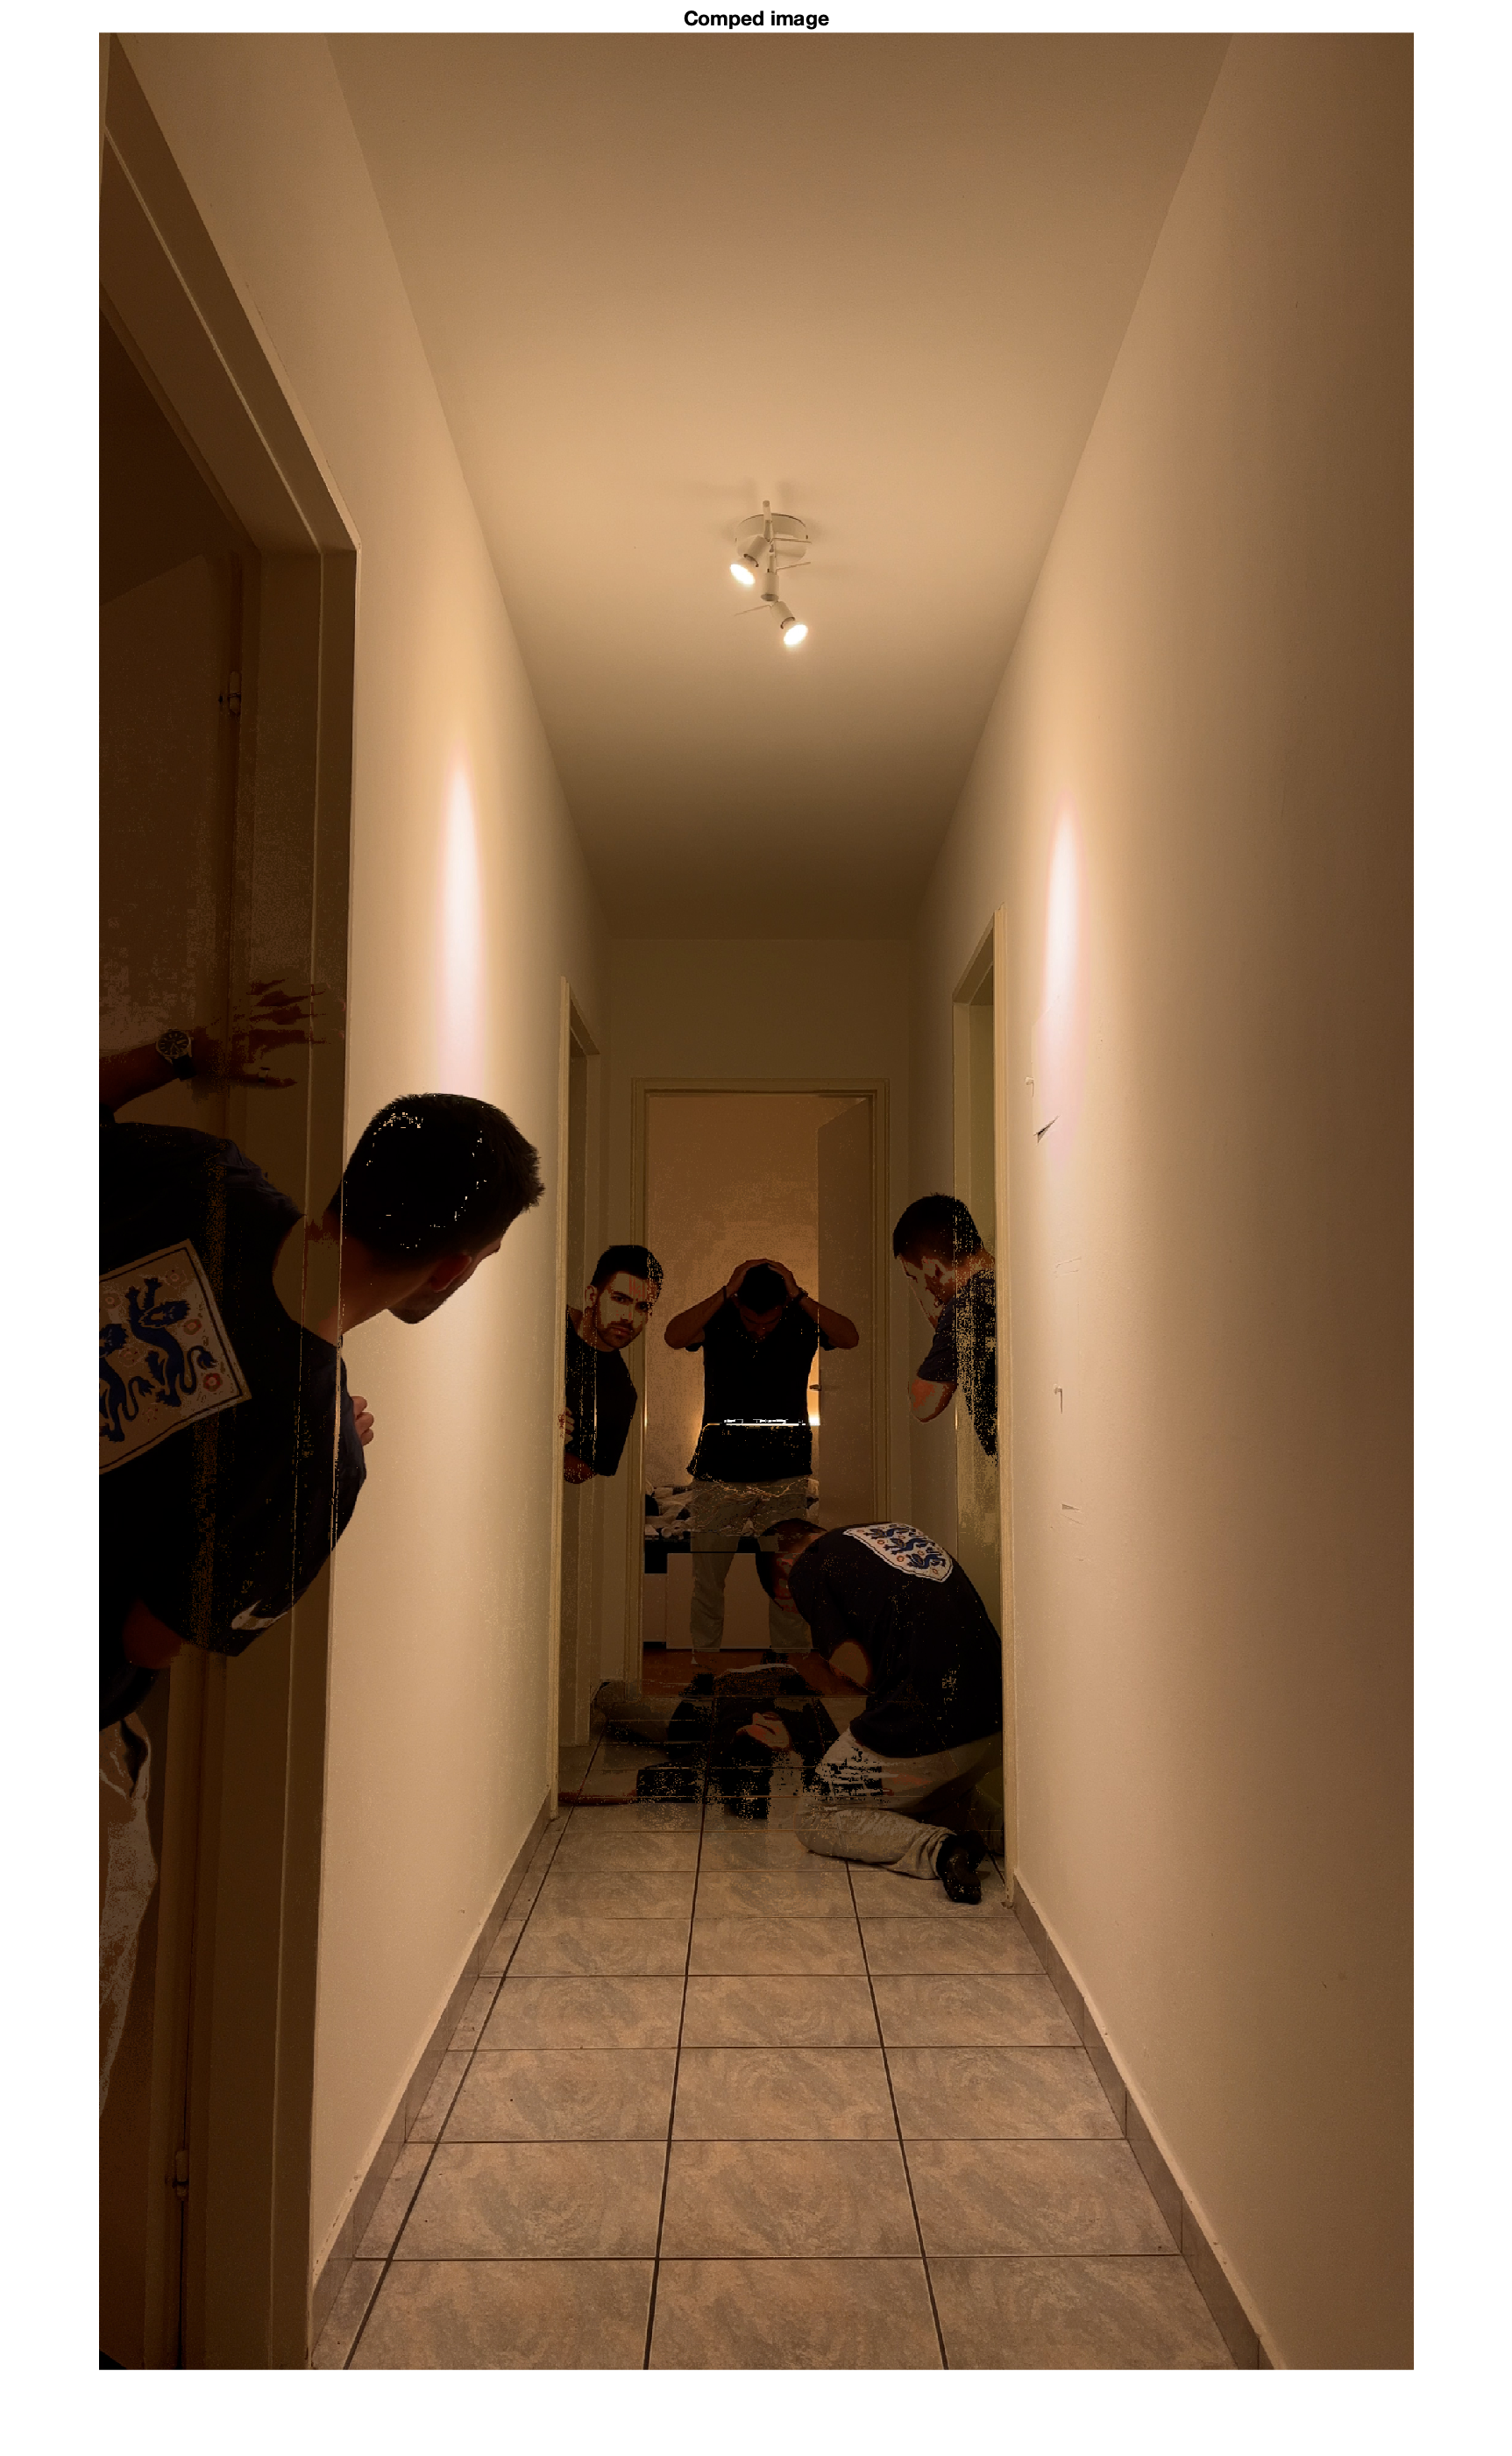
\includegraphics[width=\textwidth]{fig/out/8.im_comped.png}
        \caption{Final composited image}
        \label{fig:8.mourning}
    \end{subfigure}
    \caption{Mourning the death of Albert}

\end{figure}
\end{document}